\chapter{Method}
\label{Method}
To log and analyze network and power usage for our IoT devices, we set up an IoT testbed. This chapter documents the setup process for each IoT device, the logging process, how those two things resulted in the IoT testbed, and the software created to analyze the logged data.

\section{IoT Testbed Overview}
The flow diagram in Figure \ref{fig:network} outlines the IoT test bed constructed for this project. IoT devices pull power from the outlets through the smart switches, which log the power usage, and the WAP (Wireless Access Point) queries the smart switches for that data and pushes it to an AWS (Amazon Web Services)\cite{rds} MySQL\cite{mysql} database as an entry in the `power' table.

The wireless network provided through the WAP intercepts network packets of the IoT devices connected to it, parses them into power and network entries, and pushes them to the database. Finally, for analysis, a user can run a python script called realTimeGrapher.py, which pulls from the database and graphs this data in real time or from set intervals in the past.

Section \ref{Physical Layout and Setup} discusses the devices we used, the setup of each device, and the physical layout of the IoT test bed. Section \ref{software} covers the software part of the IoT test bed, including the usage of this test bed and what was done to obtain results for analysis.

\begin{figure}[H]
    \centering
    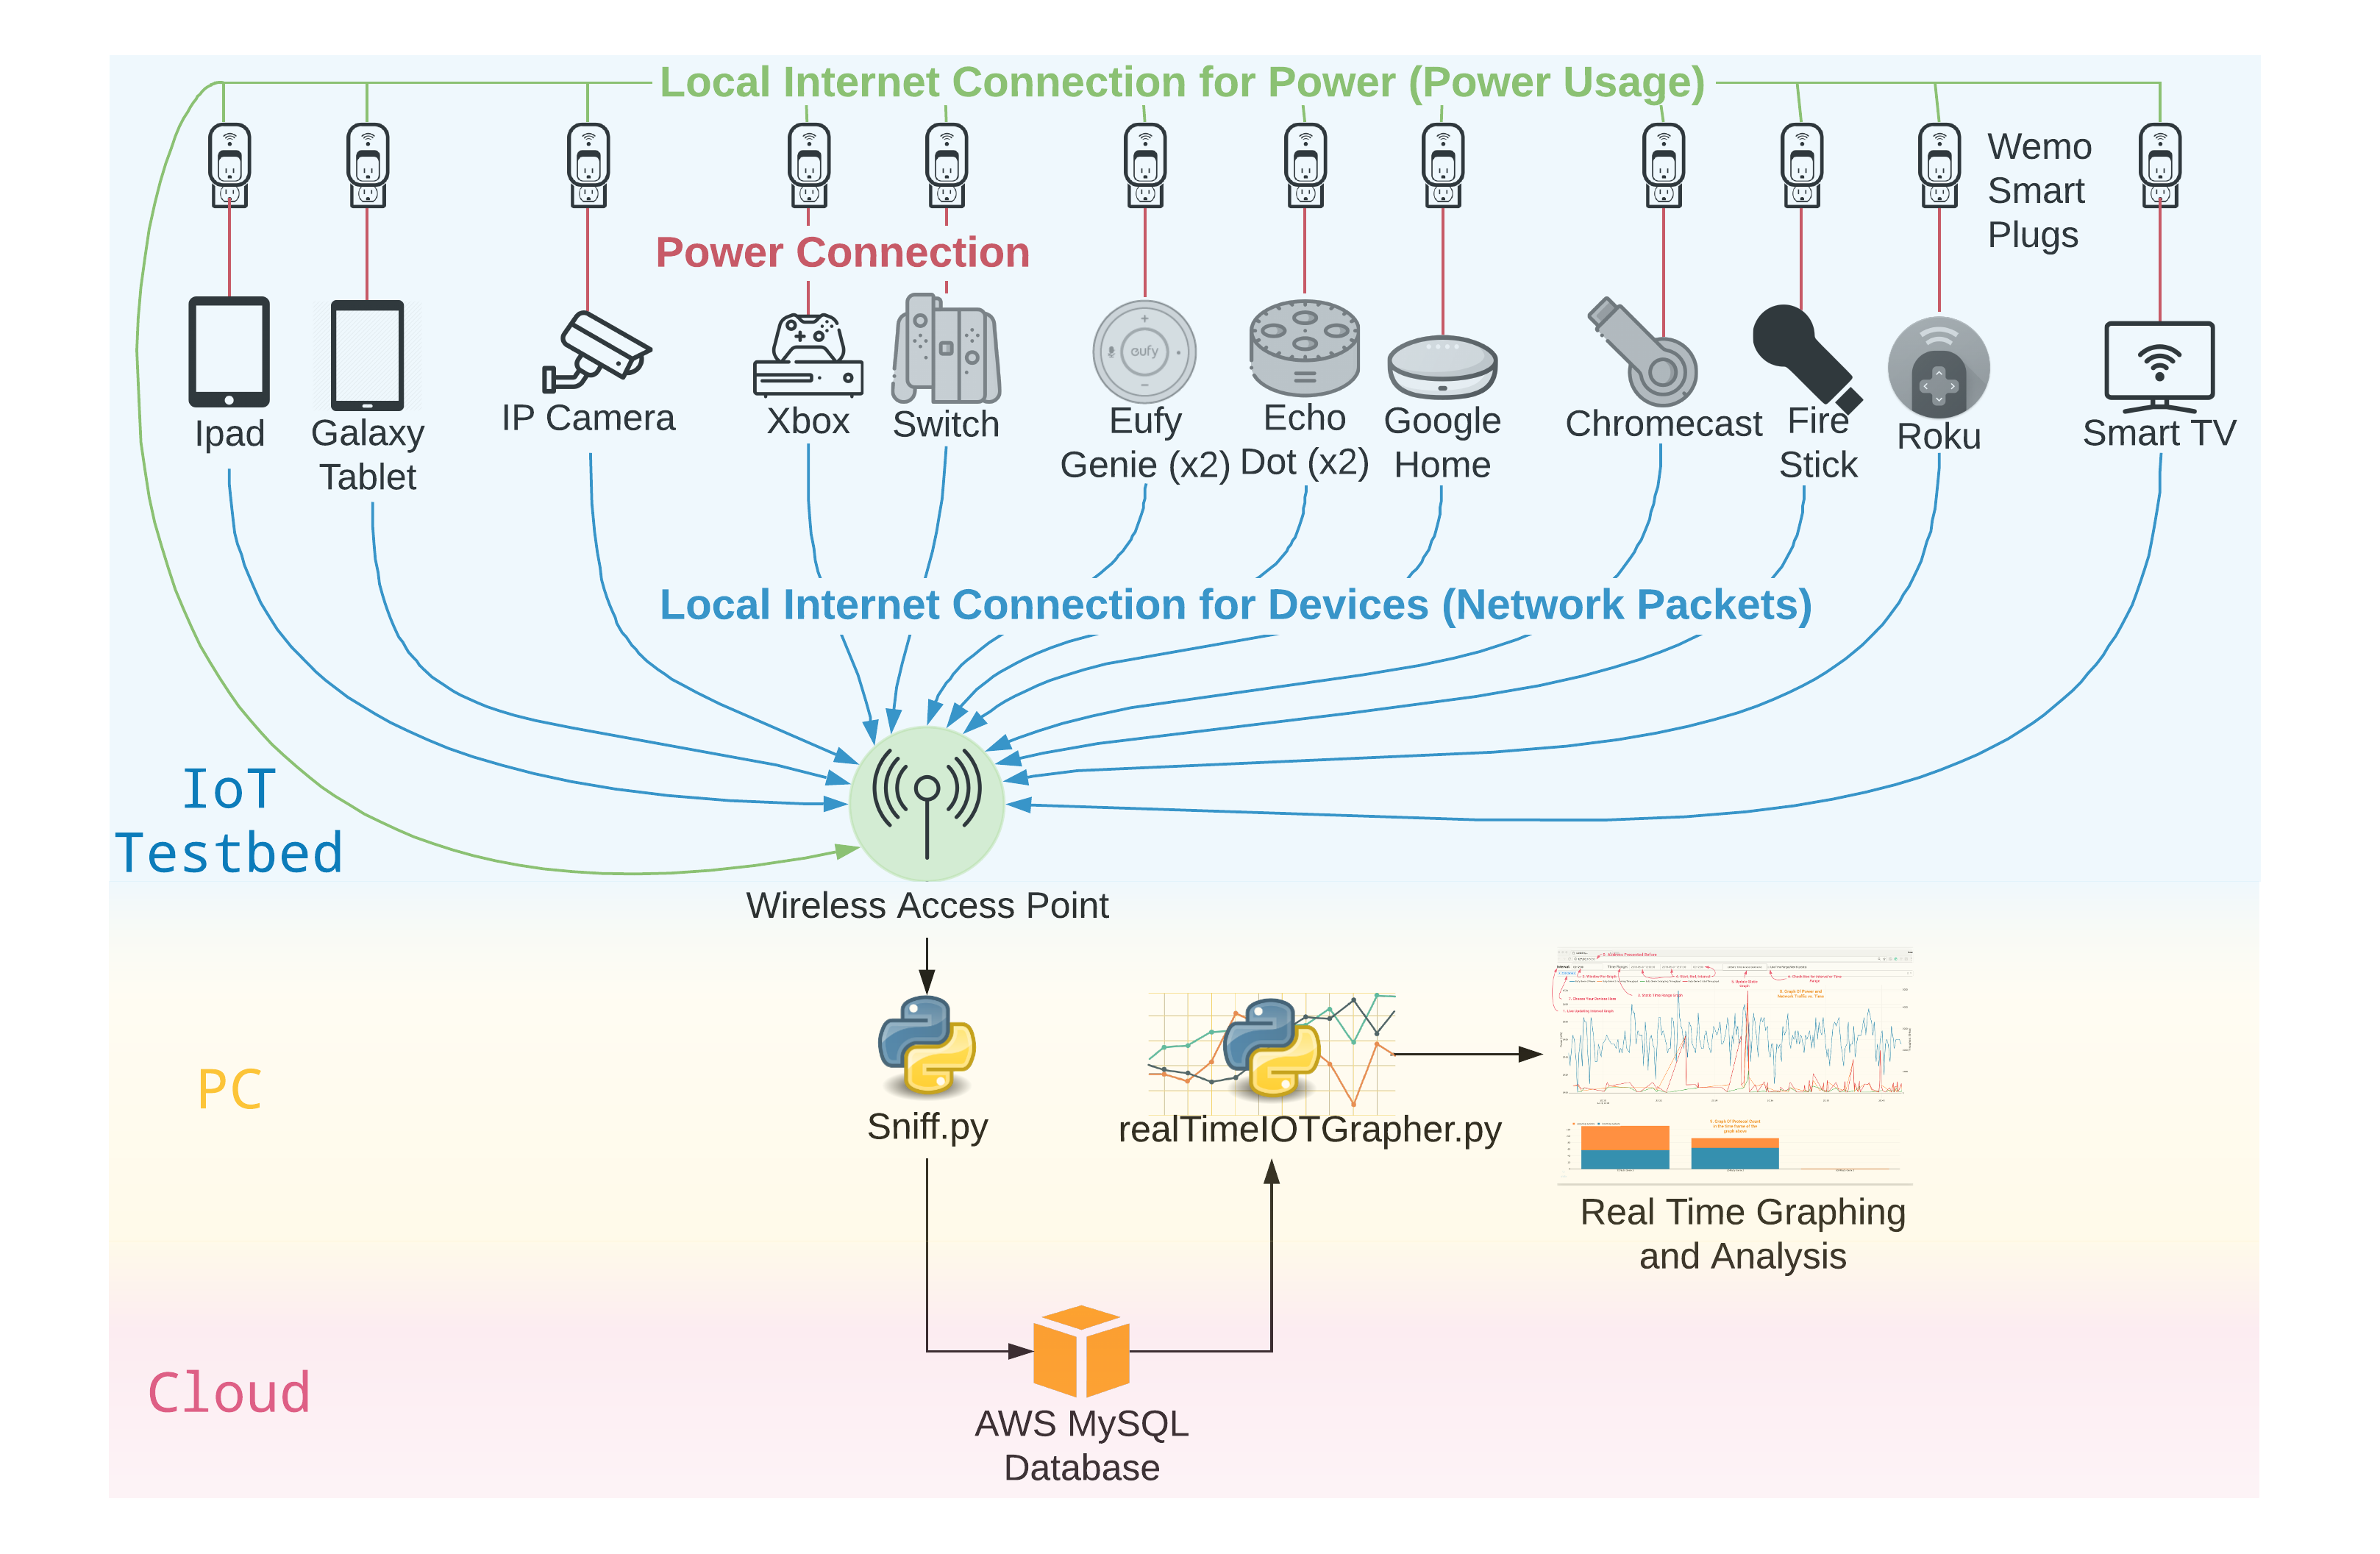
\includegraphics[width=1.0\textwidth]{networkDiagram}
    \caption{IoT testbed.}
    \label{fig:network}
\end{figure}

\begin{figure}[H]
    \centering
    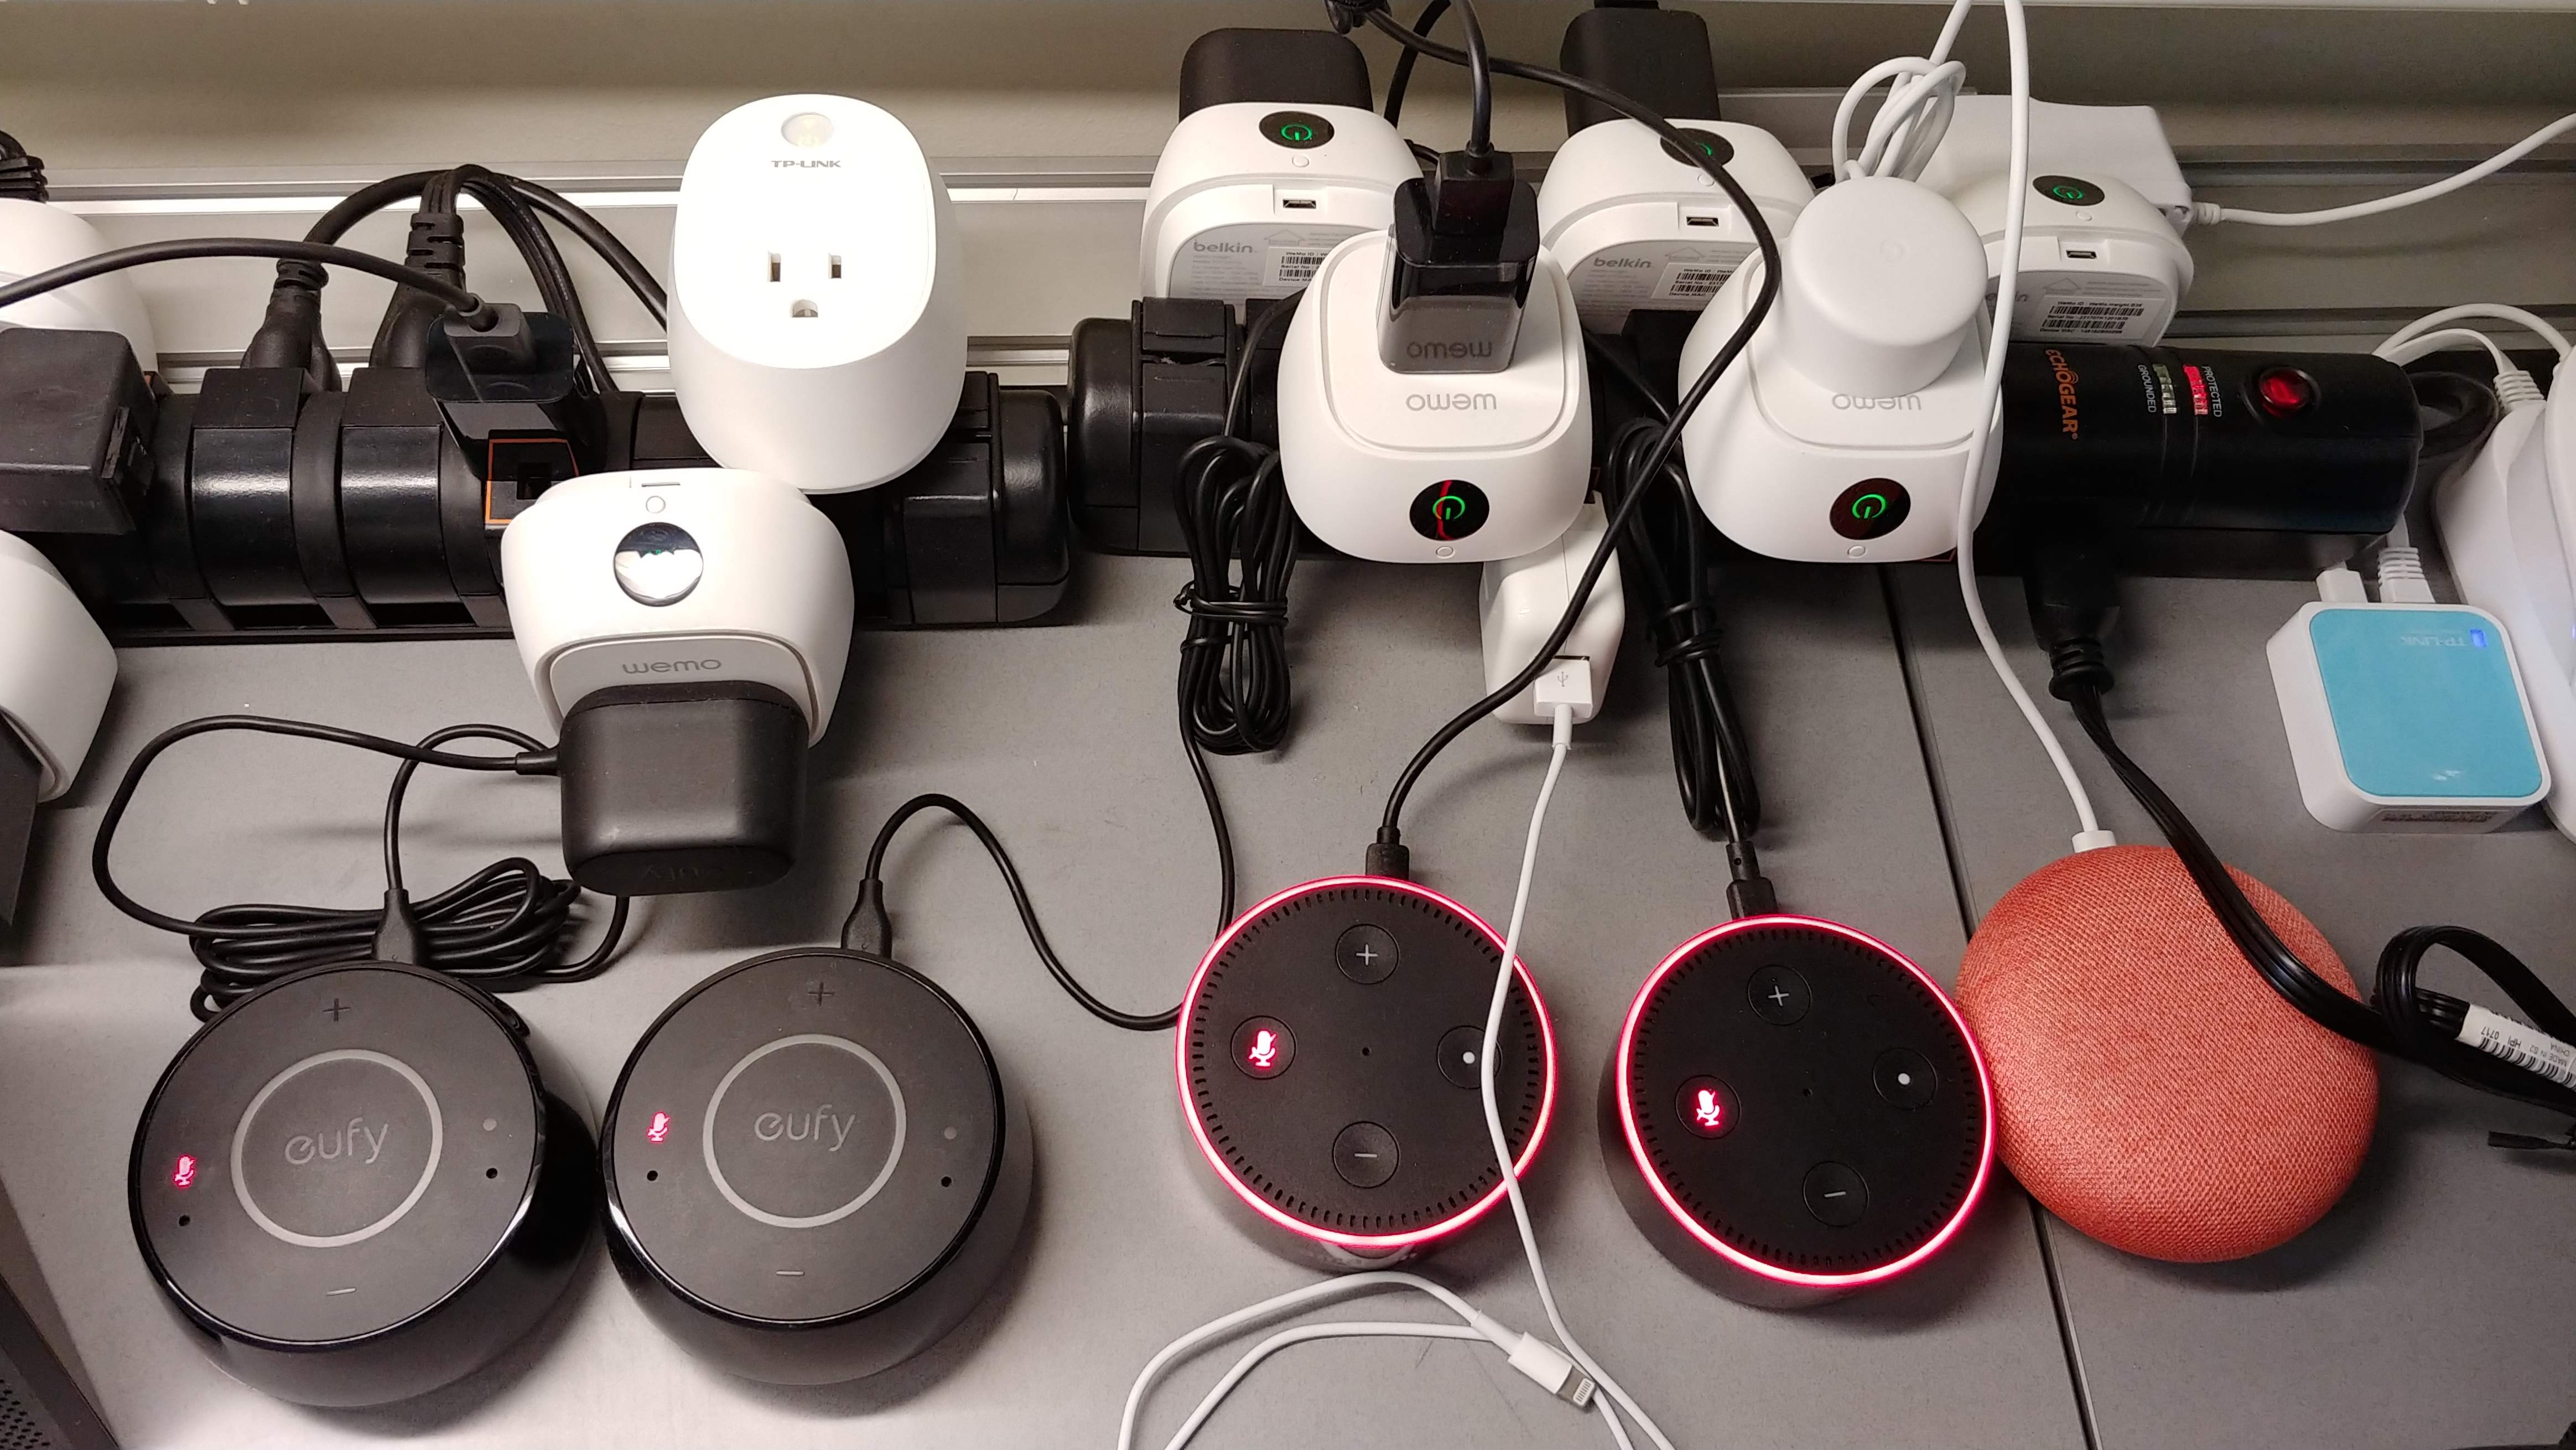
\includegraphics[width=1\textwidth]{wemos}
    \caption{Smart Speakers Connected to WeMo Insight Switches}
    \label{fig:wemo}
\end{figure}

\begin{figure}[H]
    \centering
    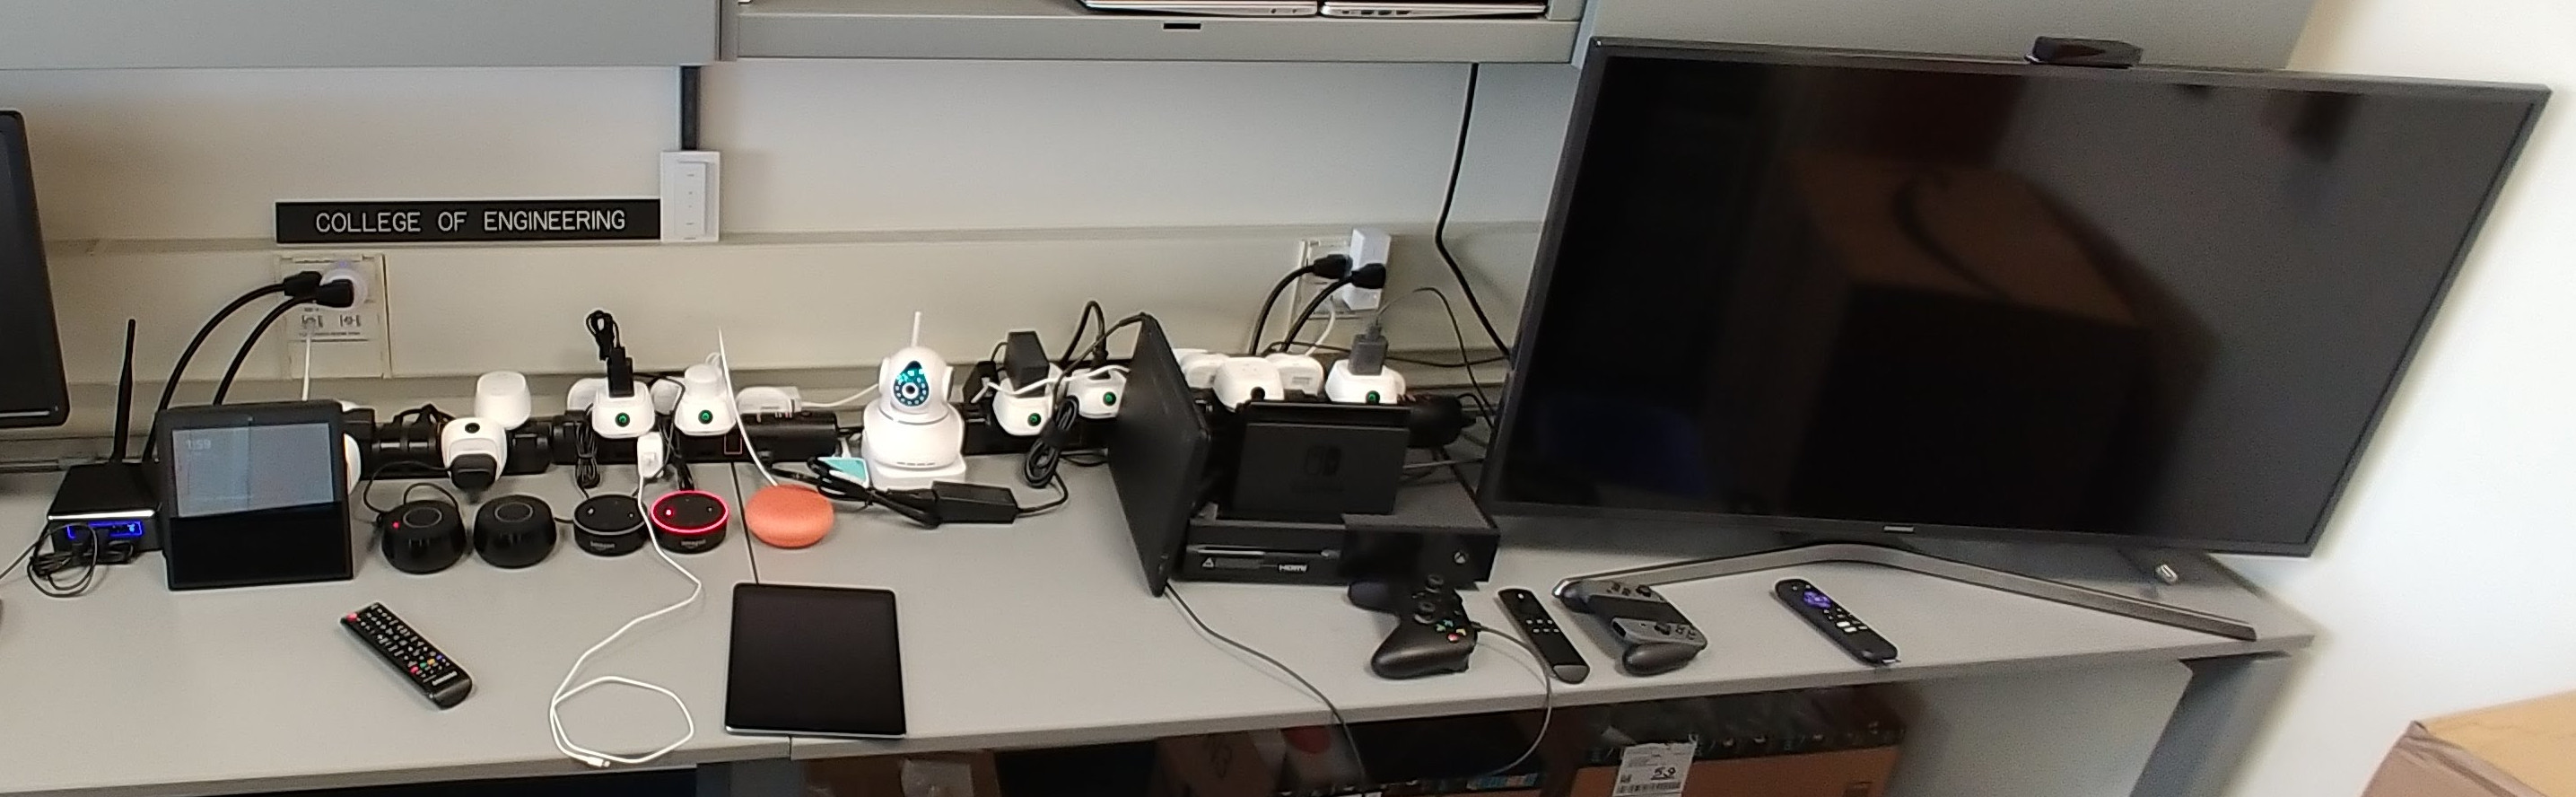
\includegraphics[width=1\textwidth]{devices}
    \caption{IoT Devices Under Examination}
    \label{fig:devices}
\end{figure}

\section{Physical Layout and Setup}
\label{Physical Layout and Setup}

This section covers the physical setup and layout of the IoT devices, and how each device is set up. Figures \ref{fig:wemo} and \ref{fig:devices} show the IoT testbed set up. Setup was performed with Ryan Frawley and explained in his master's thesis \cite{frawley_2018}; this paper provides an updated description.

\subsection{Smart Power Plugs}
Smart power plugs are pass-through outlets that can be controlled/communicate wirelessly. The outlets collect and transmit power usage over the network. They are critical to the power consumption logging in this research.

We used the Belkin WeMo Insight. We used smart outlets in general because they're affordable. We chose the WeMo insights specifically because of the Python bindings.

When setting these smart plugs up, we named each smart plug based on the device connected to it so that when we pull power information with our scripts, we can easily relate plug data to a specific IoT device. This informal naming led to issues when the wrong device is connected to the wrong smart plug, as discussed in Section \ref{realtimeIoTGrapher.py}

\subsection{Wireless Access Point}
\label{Wireless Access Point}
The wireless access point is an Intel NUC \cite{nuc}. We loaded Ubuntu\cite{ubuntu} on it because it is the most common Linux OS \cite{linux} and thus has the largest development support. The NUC was setup up as an access point that also sniffed network packets, query for power usage, and log data to a database through a Python script.

The NUC's built-in wireless interface is very slow. The throughput when using the wireless chip was measured to be 12 Mb/s down on Speedtest.net by Ookla \cite{speedtest} when connected to with a Chromebook \cite{chromebook} (for reference, the FCC defines 25 Mb/s as the minimum rate to be considered broadband \cite{fcc_2018}). This rate limitation caused many of the Belkin WeMo smart switches \cite{wemo} to drop their connection intermittently, causing gaps in recorded power data. To solve this, we added a USB wireless antenna to the NUC. This antenna improved our internet speed to 30 Mb/s down when tested on Speedtest.net by Ookla with the same Chromebook, and solved the issue of devices losing connectivity.

\subsection{Devices}
\label{Devices}
This section goes over the smart speakers, streaming devices, video game consoles, tablets, security cameras, or other devices in the IoT testbed as listed in Figure \ref{tab:devices}. These devices were included based on their popularity, as the goal of master's thesis is to build a data set from common household IoT items.

\begin{table}[H]
    \centering
    \caption{IoT Devices Being Monitored}
    \begin{tabular}{@{}llll@{}}
    \toprule
    Category & Manufacturer & Device        & Quantity \\ \midrule
    Game Console & Nintendo     & Switch        & 1        \\
    Game Console & Microsoft    & Xbox One      & 1        \\
    Laptop & HP           & Chromebook    & 1        \\
    Media Player & Samsung      & Smart TV      & 1        \\
    Media Player & Google       & Chromecast    & 1        \\
    Media Player & Amazon       & Fire TV Stick    & 1        \\
    Media Player & Roku         & Express       & 1        \\
    Security Camera & Eray    & Hi3518 Wi-Fi Camera     & 1        \\
    Smart Speaker & Amazon       & Echo Dot      & 2        \\
    Smart Speaker & Eufy/Anker   & Genie         & 2        \\
    Smart Speaker & Amazon       & Echo Show     & 1        \\
    Smart Speaker & Google       & Home Mini     & 1        \\
    Tablet & Amazon       & Fire 7 Tablet & 2        \\
    Tablet & Samsung      & Galaxy Tablet & 1        \\
    Tablet & Apple        & iPad          & 1        \\ \bottomrule
    \end{tabular}
    \label{tab:devices}
\end{table}

\subsubsection{Smart Speakers}
\label{Smart Speakers}

Smart speakers are IoT devices that combine speakers with built-in voice assistants. Some voice assistants include the Amazon Alexa, Google Assistant, or Apple's Siri. These devices are mainly controlled by voice commands, preceded by a wake word such as ``hey Google''.

Currently, around 39 million people (16 percent of the US population) use smart speakers\cite{perez_2017}. In 2022 it is projected that 70 million US households will have at least one smart speaker (55 percent of US households) and around 175 million smart speakers total\cite{perez_2018}. For these reasons, we included this group of devices in our research.

Within the smart speaker category, we included the Amazon Echo Dot, Google Home, and Eufy Genie. The Amazon Echo Dot and the Google Home are the two leading smart speaker products. We added the Eufy Genie because it is a third party Amazon Alexa device that we can compare with the Echo Dot. We also included the Amazon Show, which is a voice assistant with a screen.

\subsubsection{Streaming Devices}

Streaming devices are IoT products that connect to a television or are built into a television (smart TVs) and stream videos or music from online services. In 2017 it was recorded that 70 million US households (58.7 percent of homes) had an internet enabled device capable of streaming to a TV \cite{lynch_2017}.

The specific streaming devices we look at are the Roku Express, Amazon Fire TV, and the Google Chromecast. These devices represent three popular streaming platforms (Roku, Google Chromecast, Amazon Fire TV) that have a combined user base of over 110 million users who watch content at least once a month \cite{emarketer_2017}.

To view content from these streaming devices, we use a Samsung smart TV. This TV also as streaming capabilities which we log but do not analyze in this paper.

\subsubsection{Video Game Consoles}

Video game consoles are systems specifically built to play video games. We use two out of the three most popular gaming devices including the Nintendo Switch which sold 17.8 million units \cite{nintendo} and the Xbox One, which sold 30 million units \cite{souppouris_2016} as of January 2018.

\subsubsection{Tablets}
Tablets are mobile devices that have a touch screen, performing computer tasks, but with limited IO such as an Apple iPad, Samsung Galaxy tablet, and the Amazon Fire tablet. These devices were used for interacting with the other IoT devices, which require a smartphone or tablet for set up or control. Some of the IoT devices are limited to either Android, which runs on the Galaxy, or IOS, which runs on the iPad. Although there is no analysis on these devices in the paper, the network packets are logged. We did not track the power usage of these devices because they ran on battery power. Tracking a device's charging method as opposed to its actual power usage was out of the scope of this project.

\subsubsection{Security Camera}
Security cameras are cameras meant to run constantly as surveillance, streaming the video footage so a user can view it from any connected device at any time. Two out of the five largest recorded cybersecurity attacks targeted security cameras \cite{guest_2018}. The camera we use is the Eray camera. It has a weak username:password of admin:1234. A weak username and password make it very susceptible to cyber-attacks. There have also been reports that smart cameras have been found to send unencrypted data \cite{feamster_2016}.

\subsubsection{Other Devices}
We also connected several other devices that are harder to categorize, analyze, or both.

We have a smart hub connected to a smart lock, an indoor room temperature sensor, and smart LED light bulbs. These devices communicate with the smart hub through Zigbee or Bluetooth rather than through network packets. To look at the network traffic caused by smart lights individually, we disconnected all devices besides the smart LED bulb from the smart hub. This isolation minimized other packet noise to the smart hub. Now the smart hub's network packets should mostly be due to actions by the LED bulb because it is the only one connected to it. We performed this process a few times as one of the experiments with it. But we did no further analysis on this.

We also have a Chromebook which we used to control the Chromecast. However, because the Chromebook is more a laptop than an IoT device, we decided to leave this out of our research.

\subsection{Wiring and Configuration}
\label{Wiring and Configuration}
After obtaining all the hardware necessary, the next thing was to set up the IoT testbed. This section briefly covers WeMo Insight setup, IoT device setup, and challenges/considerations faced when setting up the IoT testbed. Frawley's paper \cite{frawley_2018} previously covered this section, refer to his paper for more details. Also, the NUC was previously acquired and setup by Ryan Frawley and other students and is not covered in this section.

It was essential to log power as soon as possible to capture a first-boot power network usage for each device. So first, before setting up the IoT devices, Ryan set up the NUC for logging. We considered setting static IPs for each device, but we decided that the average user would not set up a static IP for their device and left dynamic IPs. Some devices had already been used, so they do not contain startup information(Xbox and the Echo Dot 1).

Then, we set up each smart plug through the WeMo iOS app \cite{wemoApp}, filling in the WeMo's, username, email, network configuration, and device name. A WeMo Insight is named after the device it provides power to, e.g. the Echo Dot was given the username ``Echo Dot''.

After the logging system was set up (WeMo for power usage, NUC for network traffic and logging data to database) we began setting up each device. We set up each device with a separate email account. To do this, we made 20 AOL accounts. We used email addresses that were not under control of the manufacturer of any of the devices. For example, we did not want to use any Gmail accounts because we did not want the Google Home or Google Chromecast to perform domain-specific optimizations. When setting up AOL accounts, we also faced a limitation of the number of email accounts that could be tied to a single phone number. We used two different phone numbers to circumvent this as each phone number can is allowed 15 accounts.

We plugged each device into their corresponding WeMo. Then, each device was set up through their corresponding app. Within that process, we connected the IoT device to the NUC for WiFi and created an account for the IoT device with the emails covered in the previous paragraph.

We set up each device in waves, taking around a week to set up most IoT devices. Incremental device setup with no planned organization resulted in a messy work environment, which made it difficult to match a device to it is corresponding smart plug. After a month of data logging in a disorganized scheme, it became difficult to keep track of each device. The WeMos were also placed in an inefficient way that covered up some ports, causing us to run out of ports for new WeMos to connect to. We unplugged everything, renamed the WeMos, organized the wiring, and organized the location of each smart device resulting in the setup in Figures \ref{fig:wemo} and \ref{fig:devices}. With limited power strips, the organization helped maximize power ports. We also faced the button for each power plug towards the user so that we could quickly notice whether the power plugs were on or off.

Organization streamlined the logging process overall; debugging network and connection issues were much simpler with an ordered setup. We could quickly identify redundant devices (there are two Echo Dots and Eufy Genies), run procedures on groups of devices, and determine the corresponding smart plug for each device.

\section{Software}
\label{software}
This section covers the software components used to control the IoT test bed. It discusses the scripts for logging power and network traffic, the database information, and the python script for viewing the database.

\subsection{Wireless WAP Code}
To turn the NUC into a wireless access point, we used a create\_ap script \cite{oblique_2017}. This script takes in the desired network name, Wi-Fi password, wireless interface, and turns the NUC into a wireless access point. We later found that, with/ newer versions of Ubuntu, there is a built-in feature for creating a hotspot through a wireless interface on the device \cite{m_2016}. We used this feature to simplify the number of programs running and instead have the OS handle the hotspot. As discussed in Section \ref{Wireless Access Point} we eventually had to switch to an external antenna and rerun the script to set the USB antenna as the WAP wireless interface.

\subsection{sniff.py}
\label{sniff.py}
Sniff.py runs a thread for power logging and a thread for network logging. As each logger runs, it writes the network packets and power information to a MySQL database hosted on AWS through the python MySQL client \cite{mysqlclient} library. If the database connection is lost, the script automatically reconnects.

\subsubsection{Network Logging}
Network Logging begins by opening a socket on the wireless interfaces connected. All IP packets are sniffed through this socket connection as shown in Listing \ref{lst:sock}.

\noindent
\begin{minipage}{\textwidth}
\begin{lstlisting}[label={lst:sock},caption={Open and Read from a Socket},captionpos=b]
self.socket = socket.socket(socket.AF_PACKET, socket.SOCK_RAW, socket.htons(ETH_P_ALL))
self.socket.setsockopt(socket.SOL_SOCKET, socket.SO_RCVBUF, 2**30)
self.socket.bind((self.interface_name, ETH_P_ALL))
while True:
    packet, address = self.socket.recvfrom(MTU)
\end{lstlisting}
\end{minipage}

Once we have sniffed a packet, we can obtain the metadata from the hex dump. We preserve this hex dump in case we want to extract more information from it later. From each hex dump, we extract and store the source IP, source host, destination IP, destination host, time, size, type, protocol, source port, destination port, source host, and destination host. We explain what each fields are in Section \ref{Database}.

\subsubsection{Power Logging}
In addition to network traffic, we also log the power usage. To obtain this information, we rely heavily on the Belkin WeMo Insights.

We used the PyWemo python script \cite{pywemo} to read power usage from the WeMos once per second. This is the highest frequency we could poll for power. The WeMo is capable of reading both power and energy in mW and kW hours.

Once the script queries the WeMo for its power information, we relate the WeMo to the device connected to it by extracting the name of the WeMo. This information is used when pushing power data to our database.

One issue with PyWemo and the Belkin WeMos is that they sometimes disconnect, causing the script to miss power data. To handle this issue, the script rescans for WeMos until it finds all 16 WeMos in our testbed. The rescan code for this is shown in Listing \ref{lst:wemoRescanCode}

\noindent
\begin{minipage}{\textwidth}
\begin{lstlisting}[label={lst:wemoRescanCode},caption={Rescan if all WeMos not found.}]
    def scan_until_all_found():
        print("Discovering WeMos")
        switches = pywemo.discover_devices()
        print("Discovered {} switches".format(len(switches)))
        print(switches)
        try_num = 1

        while len(switches) < 16:
            print("Did not discover enough switches, trying again{}...".format(try_num))
            switches = pywemo.discover_devices()
            try_num += 1
            print("Discovered {} switches".format(len(switches)))

        return switches
\end{lstlisting}
\end{minipage}

\subsection{Database}
\label{Database}

To store all the results of the sniffed packets and power data, we push the data to a MySQL database hosted on an Amazon AWS server. As of writing, the database holds 172,445,929 entries that take up 184.94 GB of space. The database contains two tables, one for the network traffic and one for the power usage data. To interface with our database, we used a combination of the RealTimeIoTGrapher from Section \ref{realtimeIoTGrapher.py}, Navicat \cite{navicat}, and MySQL’s command line tool \cite{mysqlCommandline}.

\subsubsection{Network Table}
\label{Network Table}
The largest part of our database is the IP network table. It is currently 179.1 GB and contains 116,830,077 entries. It is so large because it consists of all network traffic generated over 12 months. In those 12 months, we did many high bandwidth tasks such as playing music or video. These entries contain the raw hex dump of the whole packet, which contains all the metadata plus data load, further contributing to the massive size of this table. The data table's rows represent a single packet with the columns shown in the Table \ref{tab:netcol}. The research presented in Chapter \ref{Results} primarily relies on the time, source, destination, and size fields to get network throughput over time.

\begin{table}[H]
    \centering
    \caption{Columns in Network Traffic Table}
    \begin{tabular}{@{}lll@{}}
    \toprule
    Column Number & Column Name & Data Type \\ \midrule
    1             & time        & datetime  \\
    2             & source      & varchar   \\
    3             & src\_host   & varchar   \\
    4             & destination & varchar   \\
    5             & dst\_host   & varchar   \\
    6             & protocol    & varchar   \\
    7             & type (in/out)       & varchar   \\
    8             & src\_port   & varchar   \\
    9             & dst\_port   & varchar   \\
    10            & size        & int       \\
    11            & hexdump     & longtext  \\ \bottomrule
    \end{tabular}
    \label{tab:netcol}
    \end{table}
Common SQL commands we used for our analysis include those shown in listings \ref{fig:navicatPowerQuery} and \ref{fig:navicatNetworkQuery}. The most useful commands generally required examining total throughput or device throughput using ROLLUP, shown in Figure \ref{fig:navicatRollup}.

\begin{figure}[H]
    \centering
    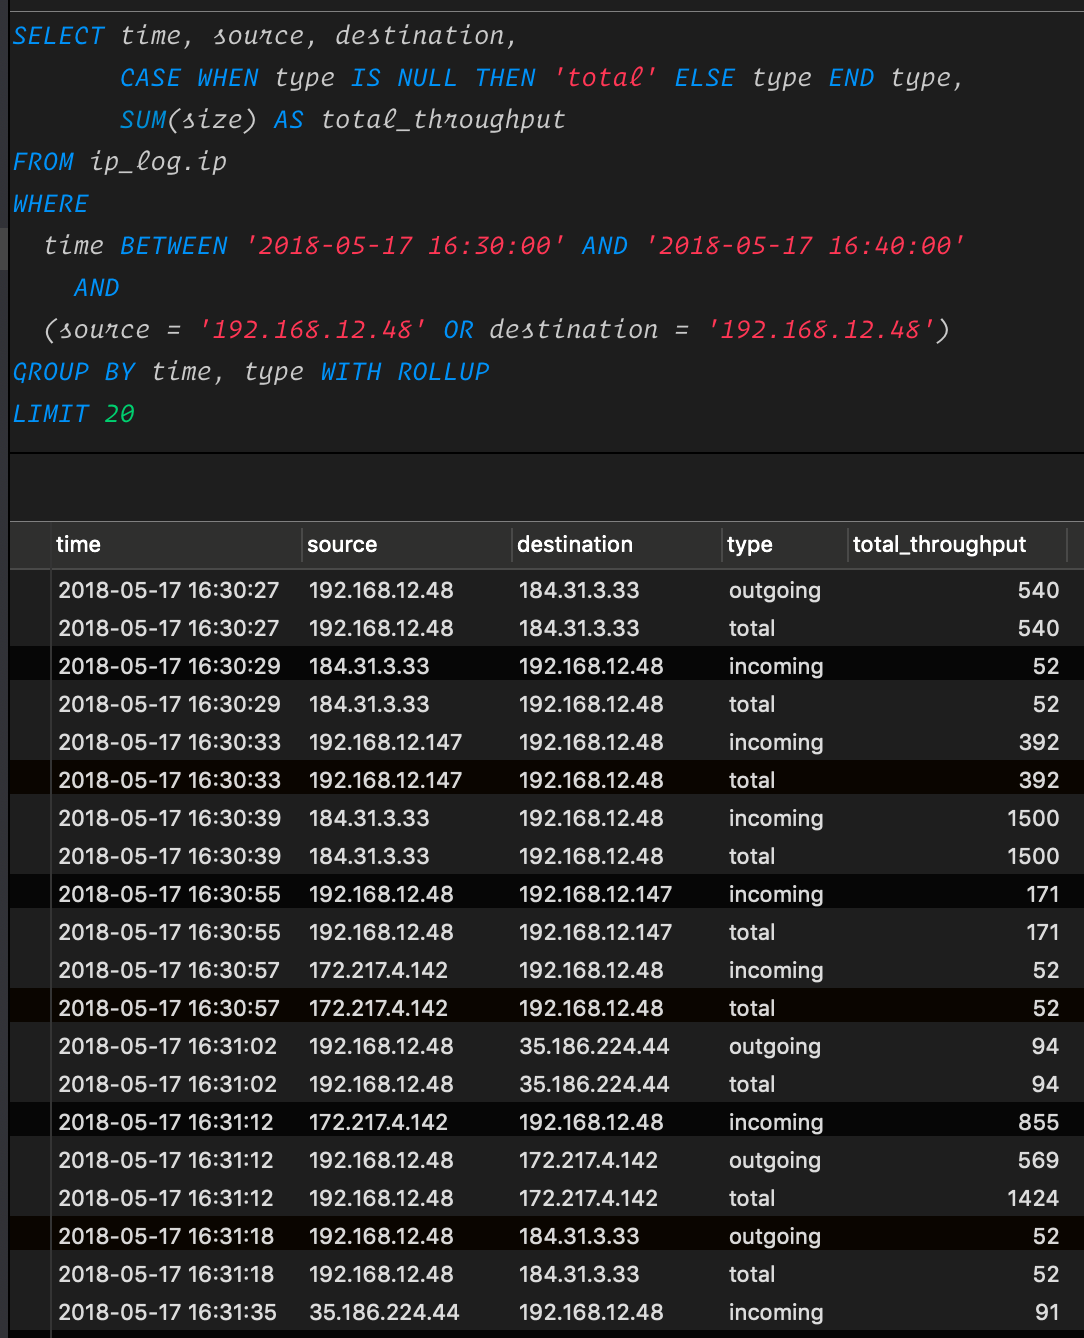
\includegraphics[width=1\textwidth]{figures/navicatRollup.png}
    \caption{Navicat IP query with rollup.}
    \label{fig:navicatRollup}
\end{figure}

The hex dump column drastically increases the size of each entry in the network table. However, as a raw network packet, it is very flexible and can be manipulated for many more use cases than the targeted columns we have. This flexibility is useful for future research that may require data we did not explicitly pull out for this project.

In the database, each device can be tracked down by looking for the IP address of that device in the source or destination columns. However, due to the use of dynamic IPs in our network setup a single device can be under multiple IPs within the table. We ignored this issue until a query for a particular IP stopped working. At which point we invoke a command on the device whose IP changed to flood the database with packets from that device, query the database in the time frame of the command, and obtain the new IP. We logged all devices and their current IP in a Google Sheets \cite{googleSheets} file covered in Subsection \ref{IP History}.

\subsubsection{Power Table}

The power table holds the most critical data for the research discussed in Chapter \ref{Results}, and I refer to it for the majority of the paper's findings. The size of this table is much smaller than the network table. It contains 5.84 GB of data and 61,240,189 entries in the database. The significant difference in size between the IP table and power table is because each device only produces one power entry every second. The columns of the power table are shown in Figure \ref{tab:powcol}.

\begin{table}[H]
    \centering
    \caption{Columns in Power Table}
    \begin{tabular}{@{}lll@{}}
    \toprule
    Column Number & Column Name     & Data Type \\ \midrule
    1             & name            & varchar   \\
    2             & power\_mw       & int       \\
    3             & time            & datetime  \\
    4             & today\_kwh      & varchar   \\
    5             & on\_for         & varchar   \\
    6             & today\_on\_time & varchar
    \end{tabular}
    \label{tab:powcol}
    \end{table}

When working with this table, we generally query for a range of power packets in a given time frame. We do this for all devices, a subset of devices, or a single device. Some of the commands and results are shown in Figures \ref{fig:navicatPowerQuery} and \ref{fig:navicatNetworkQuery}.

\begin{figure}[H]
    \centering
    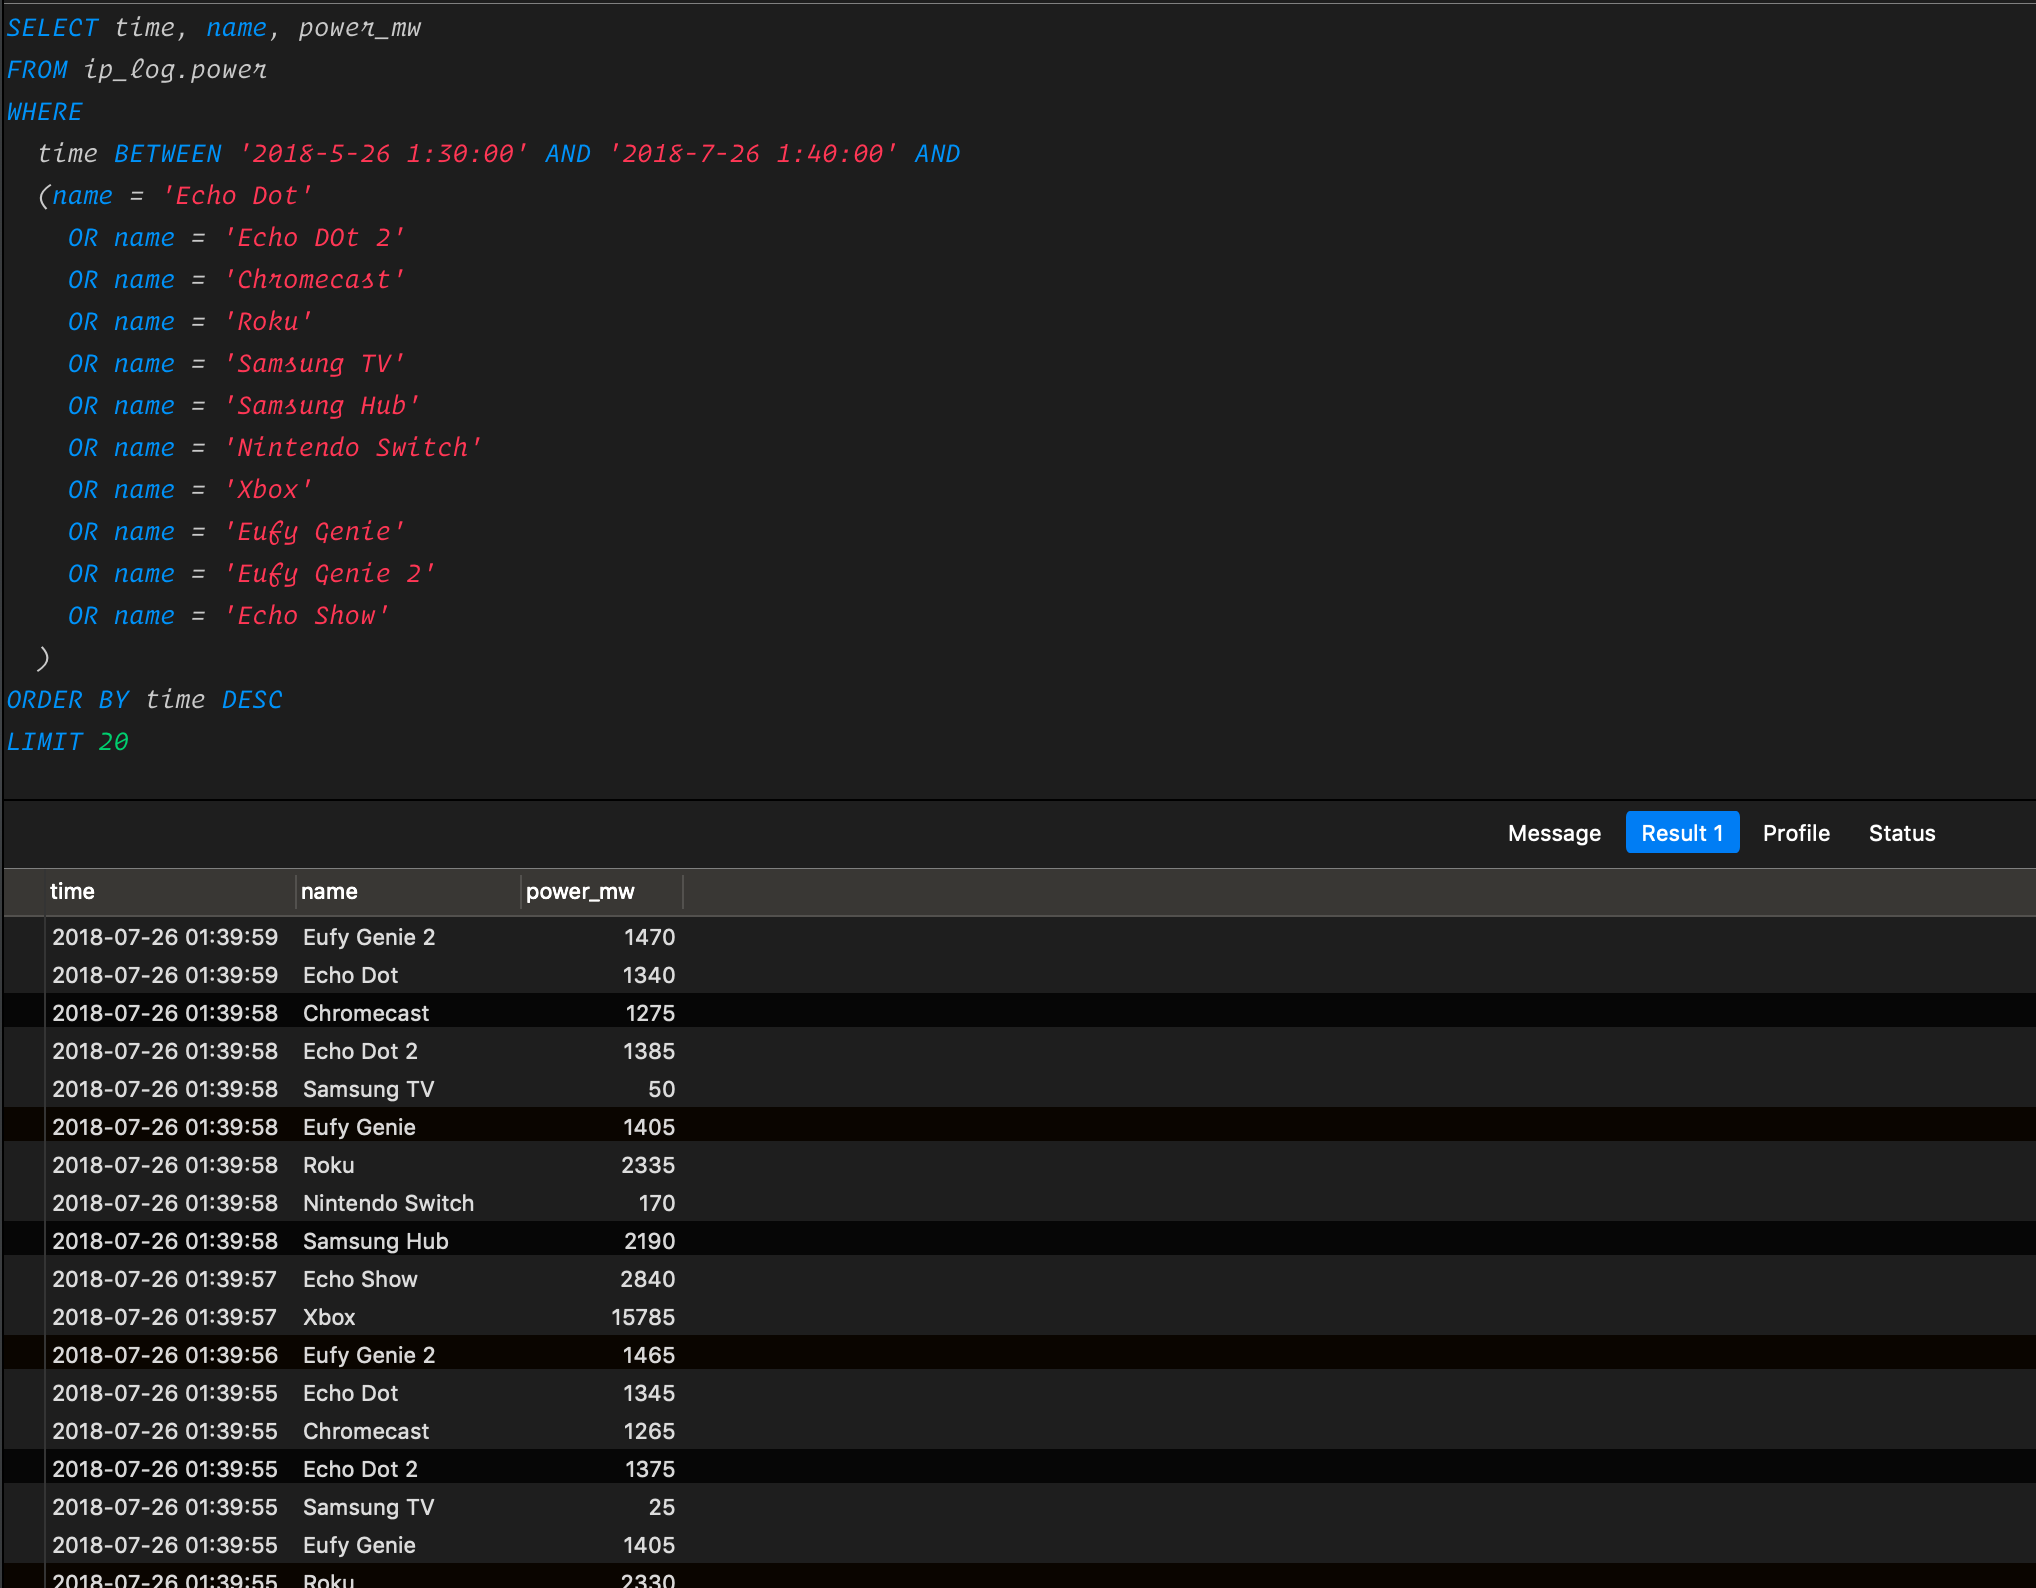
\includegraphics[width=1\textwidth]{figures/navicatPowerQuery.png}
    \caption{Power query from database with Navicat.}
    \label{fig:navicatPowerQuery}
\end{figure}

\begin{figure}[H]
    \centering
    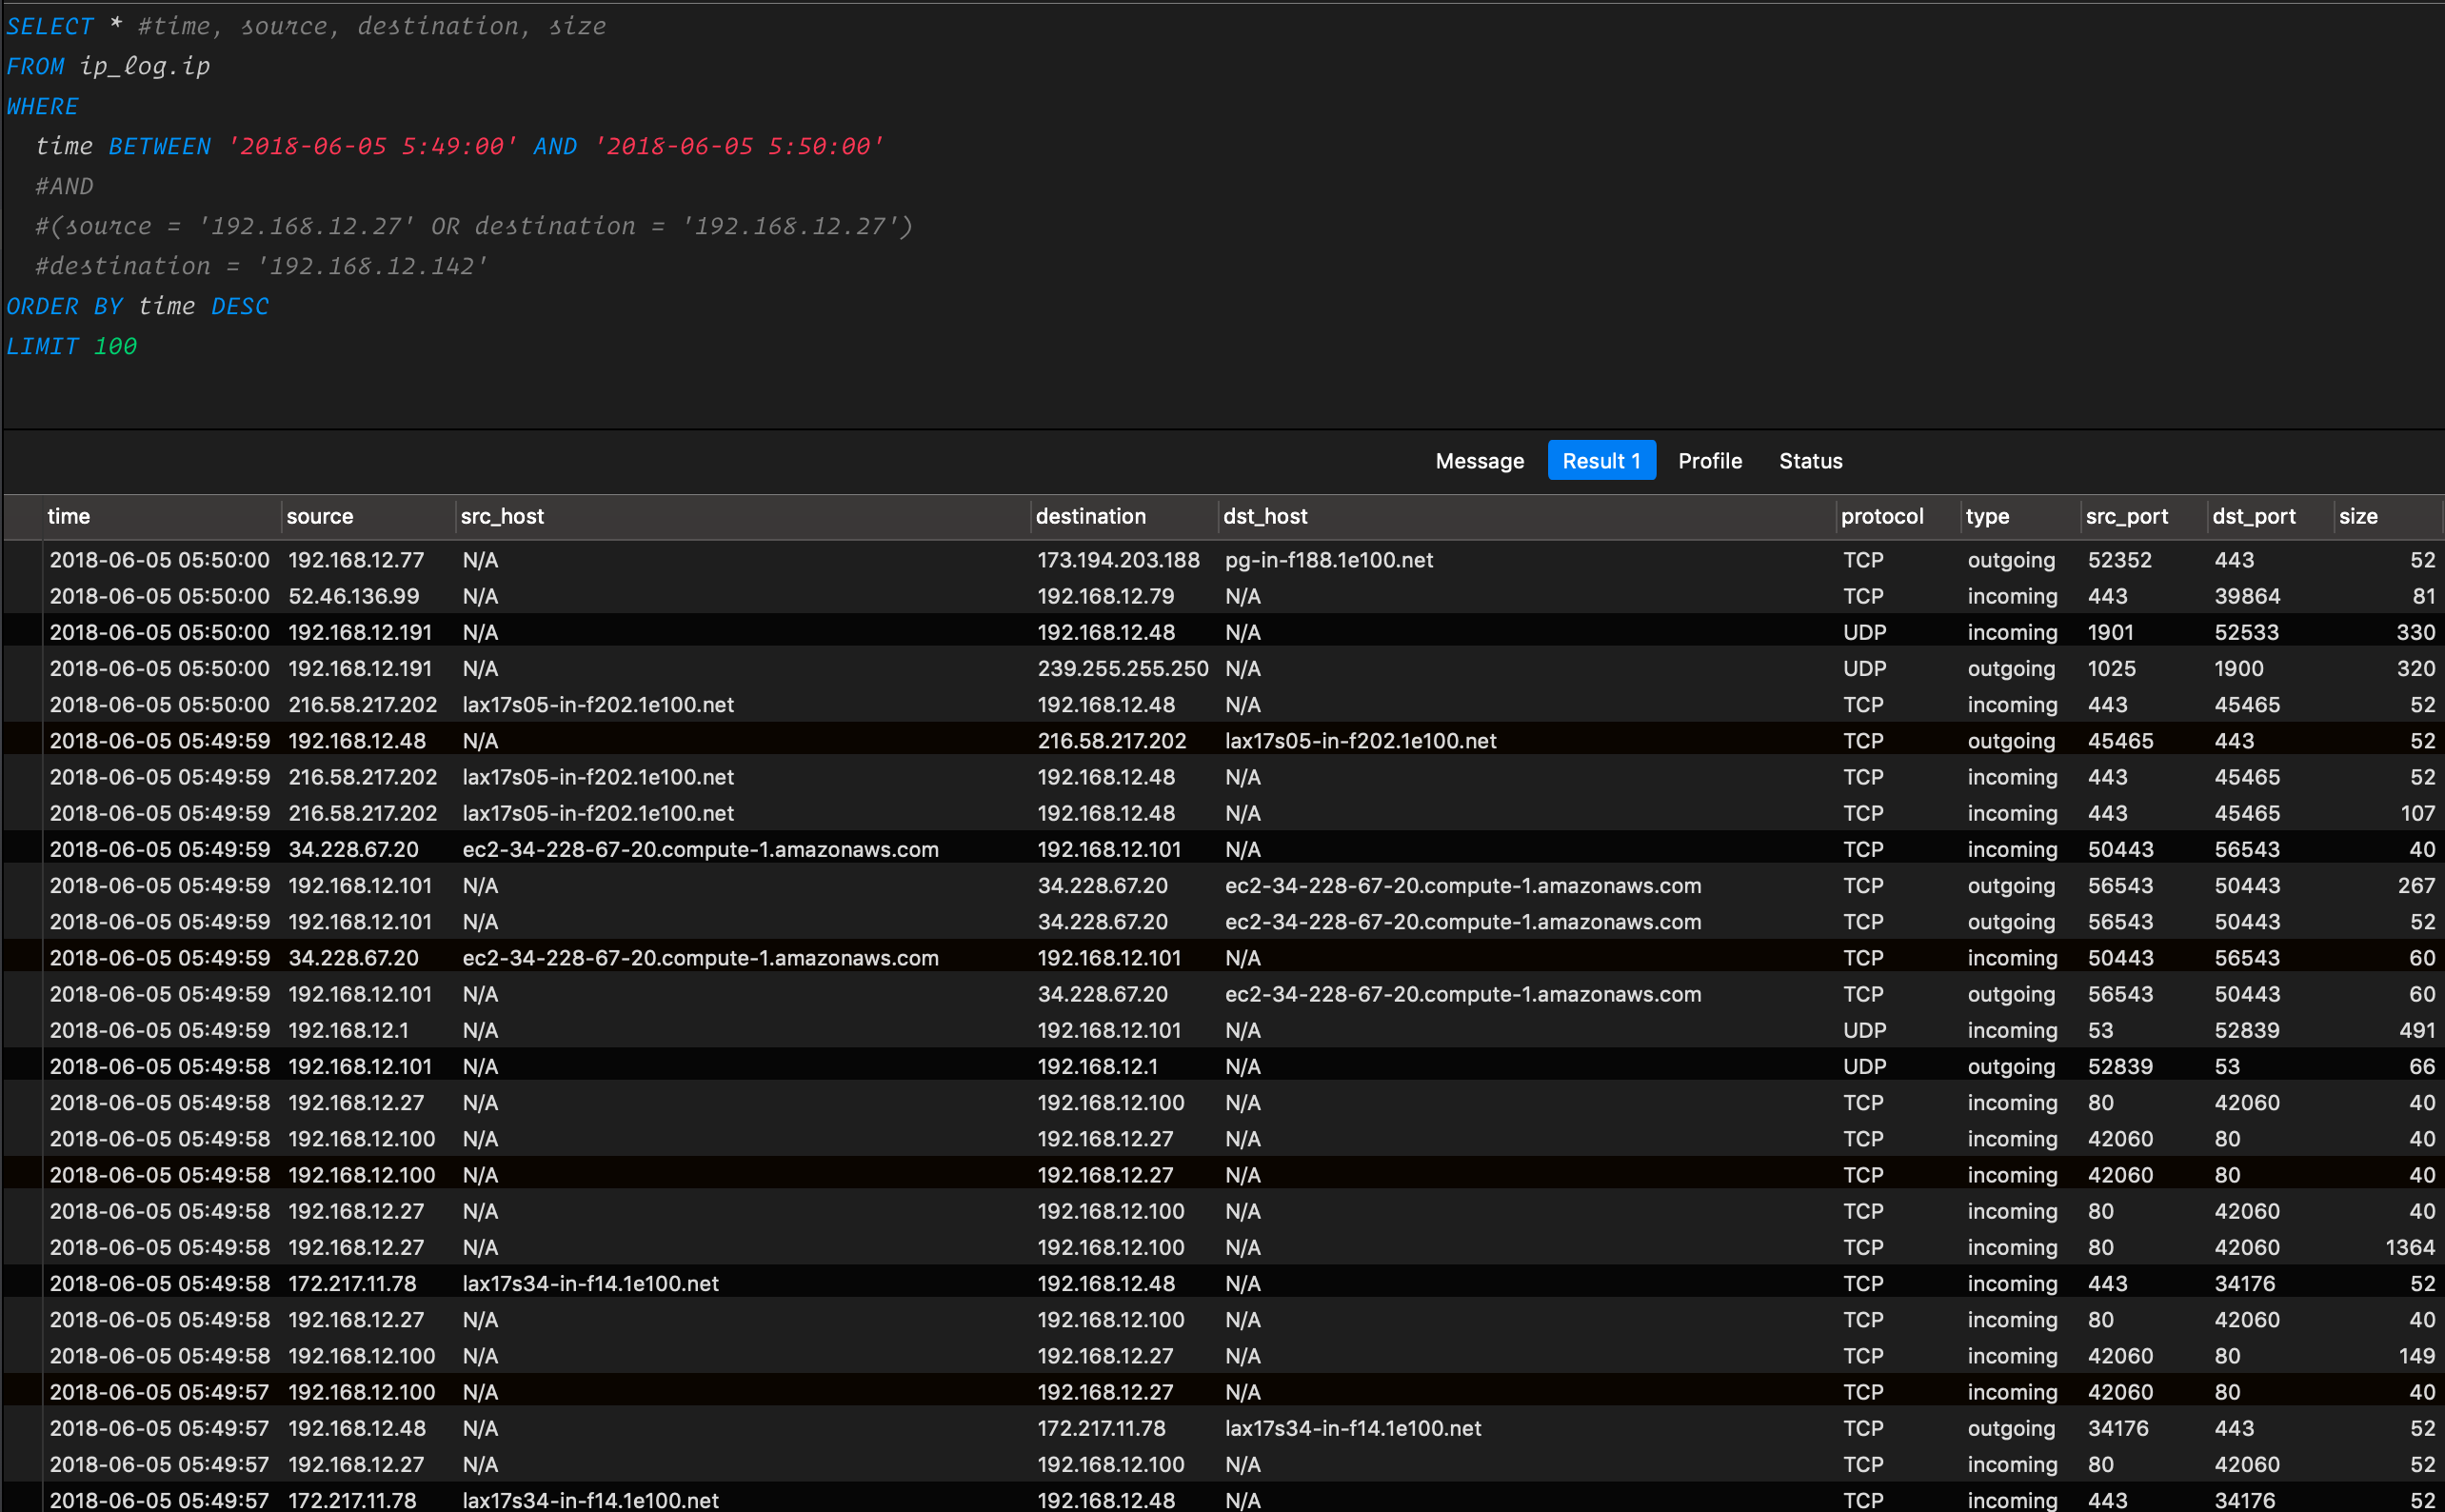
\includegraphics[width=1\textwidth]{figures/navicatNetworkQuery.png}
    \caption{Network query from database with Navicat.}
    \label{fig:navicatNetworkQuery}
\end{figure}

Within the power table, the name field is extracted from the WeMo. This can cause issues if the wrong device is connected to a WeMo. There is no way to check for this besides manual examination, which we did after a few weeks, resetting all devices and causing a temporary void in power data. Manual examination required turning the WeMo off from the iPad (where the WeMo name is displayed) and looking to see what device turned off. When we reset all devices, we also renamed some of the WeMos. For example, we changed ``echoDot'' to ``Echo Dot''. This way, all devices follow the naming convention of separating words with spaces and capitalizing each word.

The sampling frequency for the power table is also low and missing some points. Because the WeMo network connection is unstable, the script to query power data is unable to get power data every second. To handle missing points, I interpolate them as shown in Subsection \ref{realtimeIoTGrapher.py}.

\subsection{Device Inventory}
\label{Device Inventory}
To keep track of all devices and important details about them, we log a device's service, device, related email, IP address, dependencies, and password into a Google Sheets file called `Device Inventory'. An example of entries into the Device Inventory are shown in Table \ref{tab:deviceInventory}. The service field denotes the service a device provides, for example, the Google Home is a smart speaker. The device field denotes the specific manufacturer and device name. The Email and password fields denotes the email and password used when setting up the device. Some devices such as the Nintendo Switch were set up without an account. The IP address field denotes the IP address of the device within our local network. The dependencies field denotes anything the device is connected to or uses. For example, the Roku express is connected to a WeMo for power logging and comes with a controller for use.

\begin{table}[H]
    \centering
    \caption{Device inventory excerpt. Password column not shown.}
    \resizebox{\linewidth}{!}{%
    \begin{tabular}{@{}llllll@{}}
        \toprule
        Service      & Device            & Email                       & IP Address     & Dependencies     \\ \midrule
        Speaker      & Amazon Echo Dot 1 & amazonEchoDotSS0@aol.com    & 192.168.12.79  & WeMo             \\
        Speaker      & Google Home       & googleHomeMiniSS0@aol.com   & 192.168.12.48  & WeMo             \\
        Streaming    & Google Chromecast & googleChromecastSD0@aol.com & 192.168.12.78  & WeMo             \\
        Streaming    & Roku Express      & rokuExpressSD0@aol.com      & 192.168.12.68  & WeMo, controller \\
        Game Console & Nintendo Switch   & n/a                         & 192.168.12.160 & WeMo, controller \\ \bottomrule
        \end{tabular}}
    \label{tab:deviceInventory}
\end{table}

\subsection{IP History}
\label{IP History}
As mentioned in Subsection \ref{Wiring and Configuration}, the IP addresses of each device are dynamic. They change over time as DHCP assigns new IP addresses to a device. A Google Sheets file is used to keep track of each device's IP address as it changes as shown in Table \ref{tab:ipHistory}. The `Date Noticed' column is the date that the IP address was noted to have changed. The `Device' is the name of the device that changed IP address. The `Old IP' and `New IP' are the IP addresses for the device before and at that current time respectively. Newly added devices will have an `Old IP' entry as `None'.

\begin{table}[H]
    \centering
    \caption{History of IP addresses for each device}
    \resizebox{\linewidth}{!}{%
    \begin{tabular}{@{}lllll@{}}
        \toprule
        Date Noticed       & Device              & Old IP         & New IP \\ \midrule
        April 10, 2:15 PM  & Samsung TV          & 192.168.12.148 & 192.168.12.149 \\
        April 11, 2:27 PM  & Chromecast          & 192.168.12.77  & 192.168.12.78 \\
        April 12, 5:16 PM  & Fire Stick          & 192.168.12.113 & 192.168.12.114 \\
        April 20, 10:31 PM & Galaxy Tablet       & 192.168.12.222 & 192.168.12.223 \\
        April 20, 5:37 PM  & Camera              & None           & 192.168.12.57 \\
        April 24, 5:36 PM  & Home Montioring Kit & None           & 192.168.12.191 \\
        May 8, 5:59 PM     & Home Montioring Kit & 192.168.12.191 & 192.168.12.100 \\
        May 8, 6:21 PM     & Camera              & 192.168.12.57  & 192.168.12.84/83 \\
        May 18, 12:04      & Samsung TV          & 192.168.12.149 & 192.168.12.191 \\ \bottomrule
        \end{tabular}}
    \label{tab:ipHistory}
\end{table}


\subsection{Usage Flow}

One of the goals of this work is to create a data set that represents the baseline of normal network traffic and power usage. To do this, we used each IoT device at least twice a week for the year length of this research. There is a void in usage for Summer 2018 because no students were at Cal Poly to log data. To build a proper dataset that other people could use for research, we set up a list of things that we should do with each device. We logged the activities into Google Sheets so that these events could be correlated to entries in the database. For example, if someone were to look at the database and notice that the power and network traffic was high for 3 minutes, they could look at our logs and see that the device was streaming music for those 3 minutes and assume that it was normal usage.

When logging events into Google Sheets, we include the start, end time, name of the device(s), action performed, and any individual notes. When naming the devices, we use the same naming as we do for the WeMos to maintain consistency from the log to the database. An example of entries into the table is shown in Table \ref{tab:events}.

\begin{table}[H]
    \centering
    \caption{Event Log Excerpt}
    \begin{tabular}{@{}lllll@{}}
        \toprule
        Date & Start Time & End Time & Device & Event \\ \midrule
        5/25/2018 & 12:44:42 & 12:47:04 & Home Mini & Ask for news \\
        5/25/2018 & 12:55:07 & 12:56:37 & Echo Dot & Ask for news \\
        5/25/2018 & 12:55:57 & 12:56:17 & Echo Show & Ask for weather \\
        5/25/2018 & 12:56:44 & 13:03:07 & Home Mini & Play music \\ \bottomrule
        \end{tabular}
    \label{tab:events}
\end{table}

The following subsections explains the script created to automate the event logging portion of the research. Then it explains the specific procedure we ran each group of IoT devices through whenever we used them.

\subsubsection{Google Sheets Script}

Logging information into the spreadsheet is a tedious task, especially when trying to analyze each device while running tasks on them. To minimize human error, I created a script in Google Sheets to automatically populate the date and time an entry is added. The code for the script is shown in Listing~\ref{lst:sheetScript}.

\noindent
\begin{minipage}{\textwidth}
\begin{lstlisting}[basicstyle=\linespread{0.95}\ttfamily, language=C,label={lst:sheetScript},caption={Open and Read from a Socket}]
function onEdit() {
  var s = SpreadsheetApp.getActiveSpreadsheet().getSheetByName("Event Log");
  var r = s.getActiveCell();
  var c = r.getColumn();

  if( c == 4 || c == 5) { // checks the column
    var dateCell = r.offset(0, -3);

    if( dateCell.getValue() === '' ) {// is empty?
      var startTimeCell = r.offset(0, -2);

      // fill in the start time and date
      var date = new Date();
      dateCell.setValue(date);
      startTimeCell.setValue(date.toLocaleTimeString());
    }
  }

  if( c == 6 ) { // checks that the description is being entered
    // if so fill in the end time
    var endTimeCell = r.offset(0, -3);

    if ( endTimeCell.getValue() === '' ) {
      endTimeCell.setValue(new Date().toLocaleTimeString());
    }
  }
}
\end{lstlisting}
\end{minipage}

\subsubsection{Smart Speakers}
Whenever interfacing with these devices, we queried for the weather and the news. The specific phrases we used were ``$<$wake word$>$ what's the weather'' and ``$<$wake word$>$ what's the news'', we  set a reminder for a random task in a random timeframe, and we muted the devices for a few minutes to see if they were still listening if we said the wake word.

\subsubsection{Video Game Consoles}
When interfacing with these devices, we played a game on the device for at least 15 minutes. Every week, we also browsed for games on the game store and downloaded free demos.

Afterward, we turn off the Xbox and put the Nintendo Switch into sleep mode. The Nintendo Switch was only set to sleep because it can only shut down when disconnected from the dock.

\subsubsection{Streaming Devices}
When interfacing with these devices, we watched YouTube for at least three minutes.

For the Chromecast, we cycled through different devices to cast videos from, including the iPad and the Chromebook. We wanted to get varied data in case the Chromecast prioritized streaming from different devices.

\subsubsection{Tablets}
In this experimental setup, we used the tablets less for investigative purposes, but more to set up and interface with other devices.

However, we still tracked the data and had a small set list of things to do on these devices. We used each tablet to browse the web, watch YouTube, and use various apps.

\subsubsection{Security Camera}

The only security camera we worked with was the Eray Security Camera.

Whenever interfacing with this device, we used the device through the app NVAS2 \cite{nvas2} on the iPad for at least 2 minutes. Usage included streaming video from the camera to iPad to view it. We also controlled the camera through the app with pan and tilt commands. When done experimenting with the security camera, we disconnected the tablet from the camera by using the ``end stream'' button in the NVAS2 app.

\subsection{realtimeIoTGrapher.py}
\label{realtimeIoTGrapher.py}

This section covers a visual tool I created to look for trends. Originally, for trend analysis, we queried the database for the necessary data, copied the data over to Google Sheets, created the necessary formulas, graphed the network and power usage over time, and finally analyzed this graph. The tables and formulas are shown in Figure \ref{fig:excelLogging}. This process was tedious and time-consuming because we had to manually format an SQL query, entering unique time values and the IP address of the device. Copying large datasets from SQL into Google Sheets also causes lag in the browser.

To address these problems, I created a Python script that automatically forms graphs, including the one shown in figure, \ref{fig:interpolated} when given a time range and the desired devices. This automation sped up the analysis process and provided extra features covered in Section \ref{Features}.

This Python script leverages the Plotly \cite{plotly} library, which, given data, graphs it onto a local web page for viewing. Plotly comes with many useful tools for further analysis and can be extended to run on a public web page for public viewing.

I plan to distribute this tool with our database so that researchers can view the power and network information of any device at a glance.

\begin{figure}[H]
    \centering
    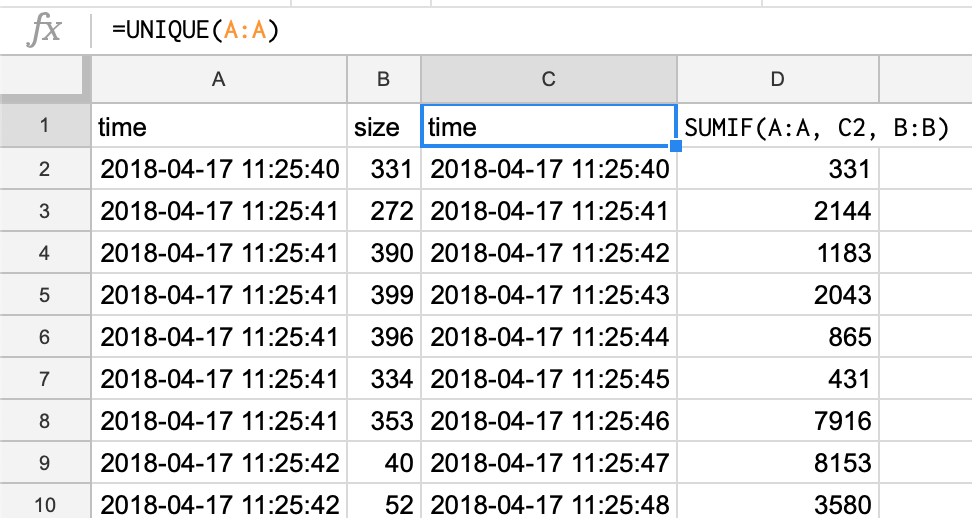
\includegraphics[width=1\textwidth]{excelLogging}
    \caption{Manual Analysis of IoT devices in Google Sheets: Raw data shown in columns A and B are then formatted into columns C and D for Graphing}
    \label{fig:excelLogging}
\end{figure}

\begin{figure}[H]
    \centering
    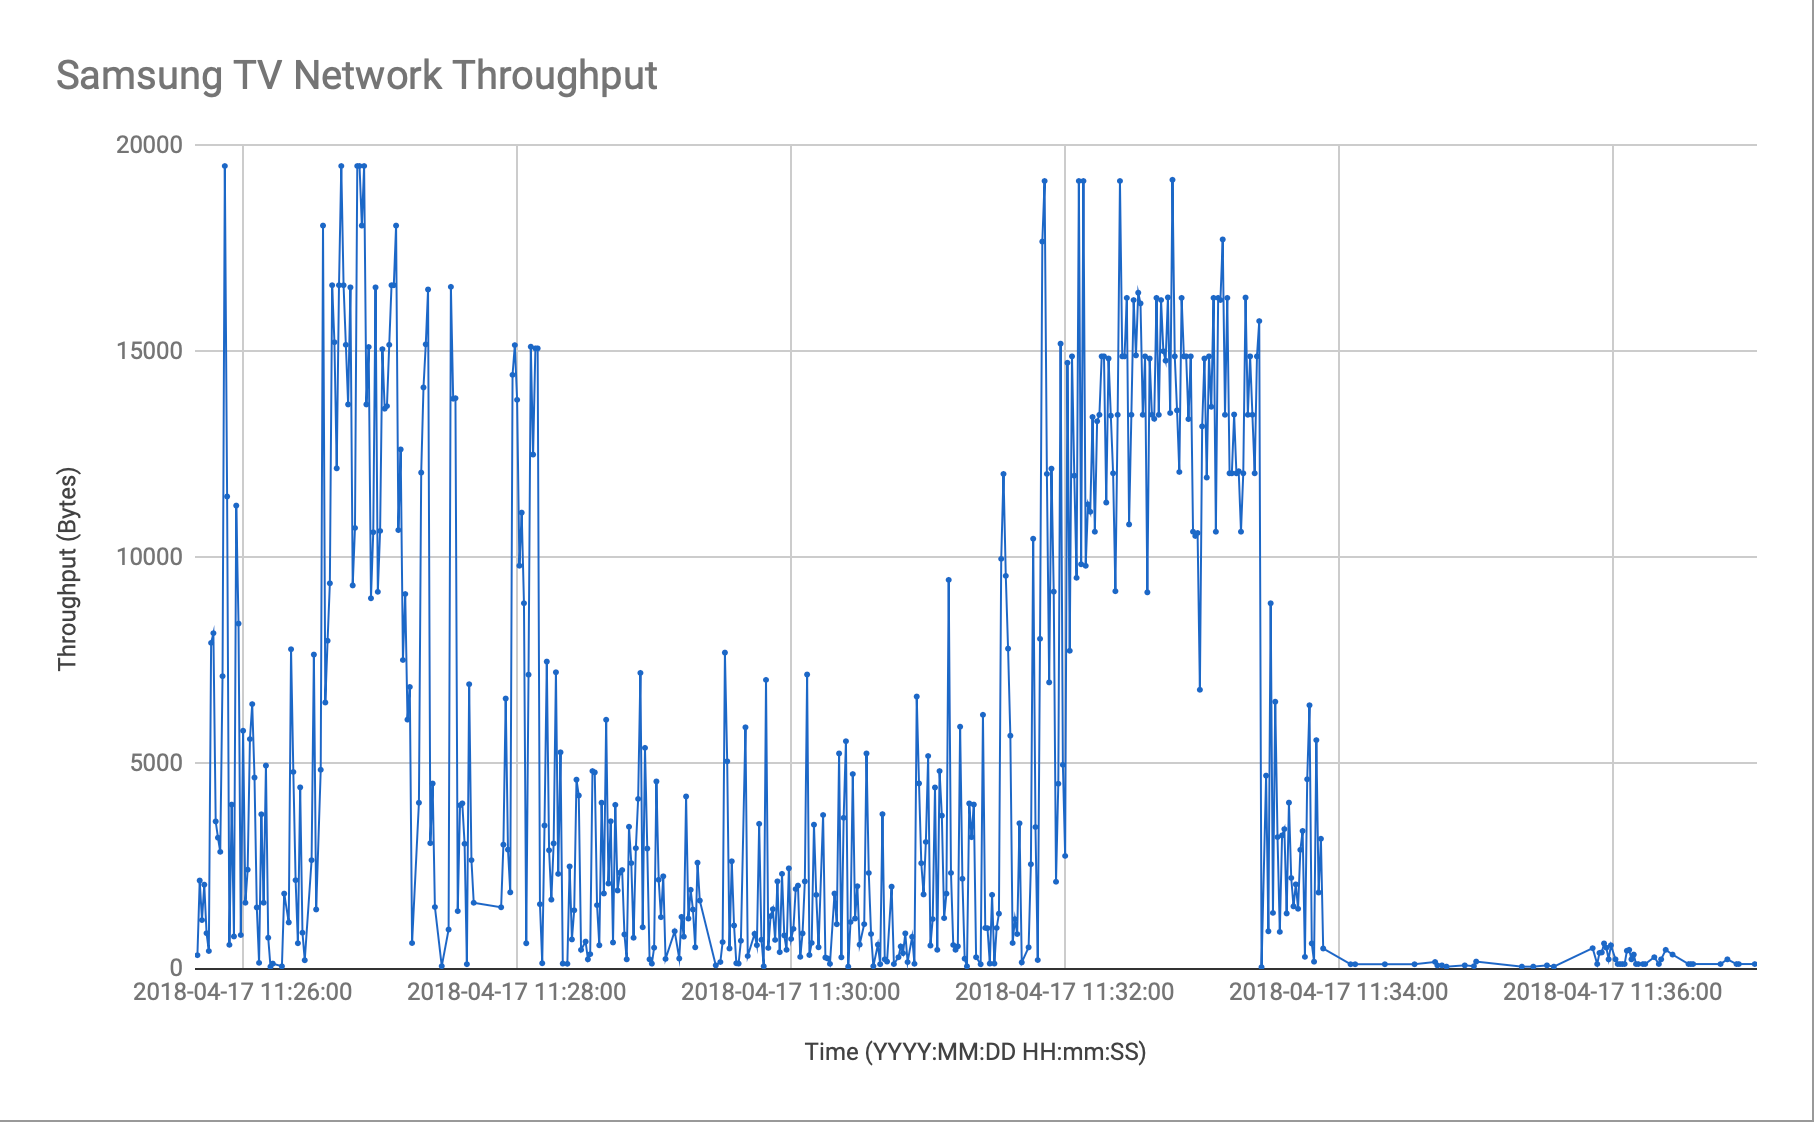
\includegraphics[width=1\textwidth]{figures/tvThroughput.png}
    \caption{Resulting graph of dataset shown in Figure \ref{fig:excelLogging}}
    \label{fig:tvThroughput}
\end{figure}

\subsubsection{Features}
\label{Features}

This section discusses the features that RealTimeIoTGrapher (grapher) provides.

At its core, this program automates the creation of the graph shown in Figure \ref{fig:tvThroughput}. The user can specify a time range that the graph should cover and what devices to graph. By default, the graph shows power, input traffic, output traffic, and total network traffic over the time range specified.

The grapher also annotates the data by including a line denoting the average for each of the traces over the time range currently displayed. It also annotates the maximum and minimum values in the time range for each trace. The grapher can also display information in real time for any specified window size (update live showing ten minutes at a time), updating every second.

The Plotly libraries also provide useful tools when displaying these IoT graphs. It is possible to zoom in and out the displayed graph, select specific traces for viewing, save the graph, and hover over data points to display the specific value. Finally, once a graph is saved as shown in Figure \ref{fig:plotlySave} Plotly allows further editing of the graph so that it is formatted the way the user wants as shown in Figure \ref{fig:plotlyEdit}.

\begin{figure}[H]
    \centering
    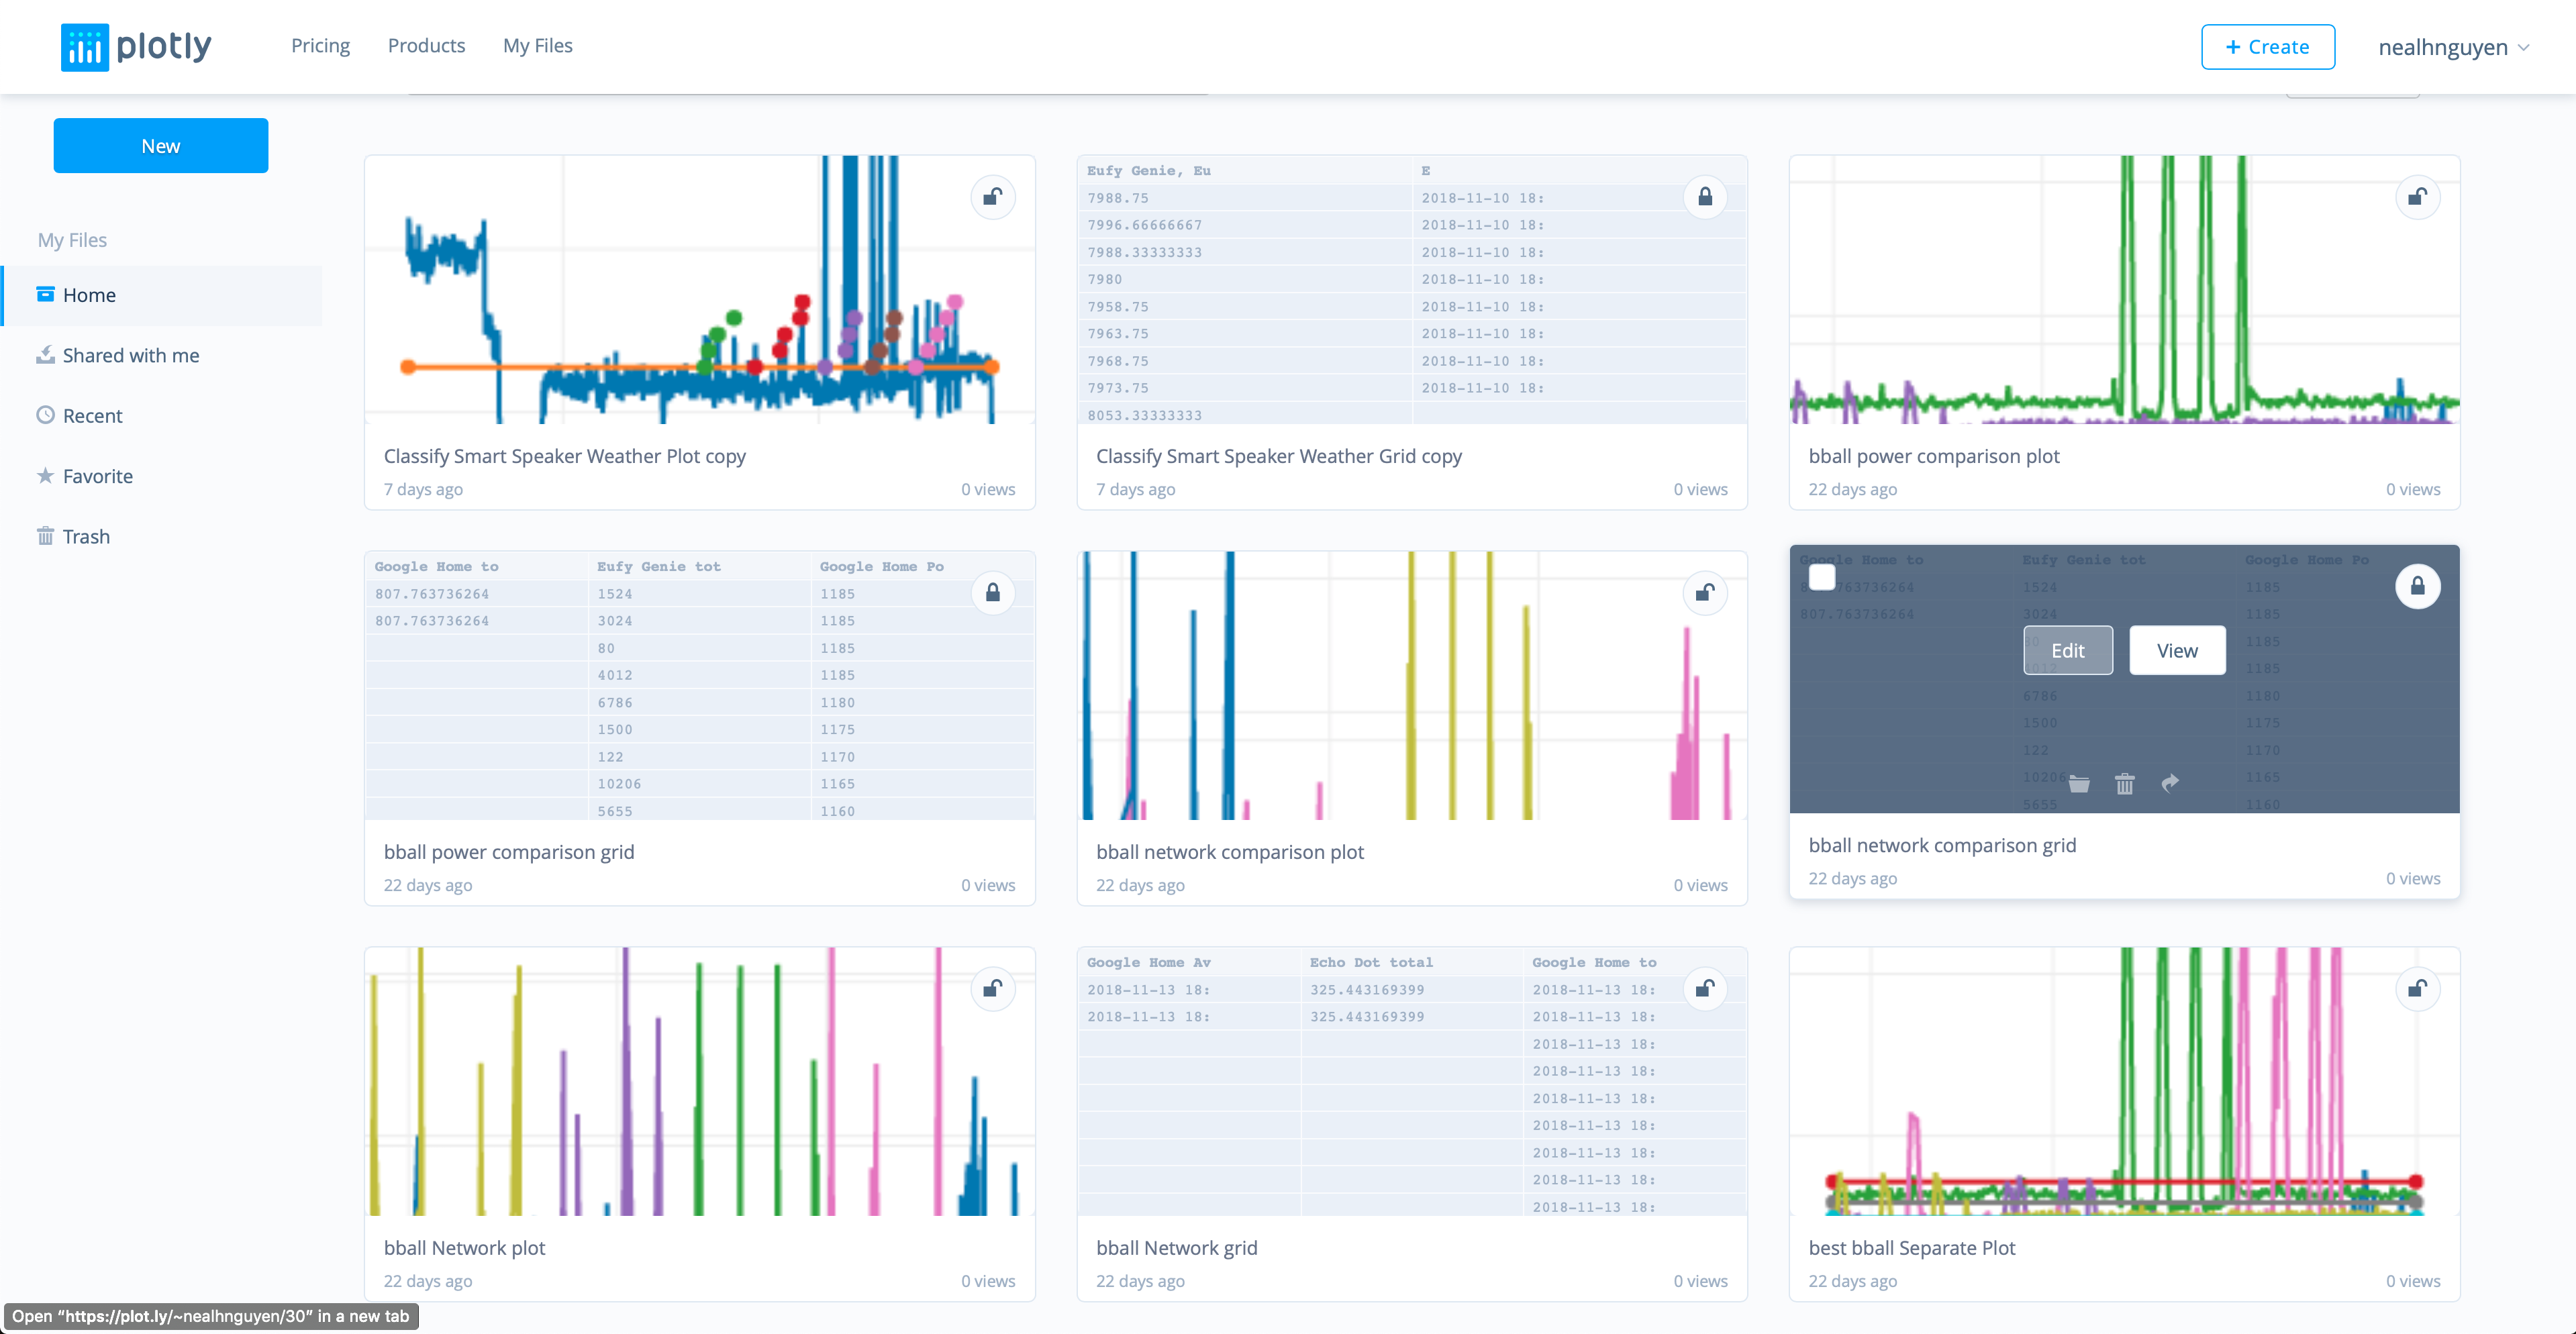
\includegraphics[width=1\textwidth]{figures/plotlySave.png}
    \caption{Screen of saved plotly graphs.}
    \label{fig:plotlySave}
\end{figure}

\begin{figure}[H]
    \centering
    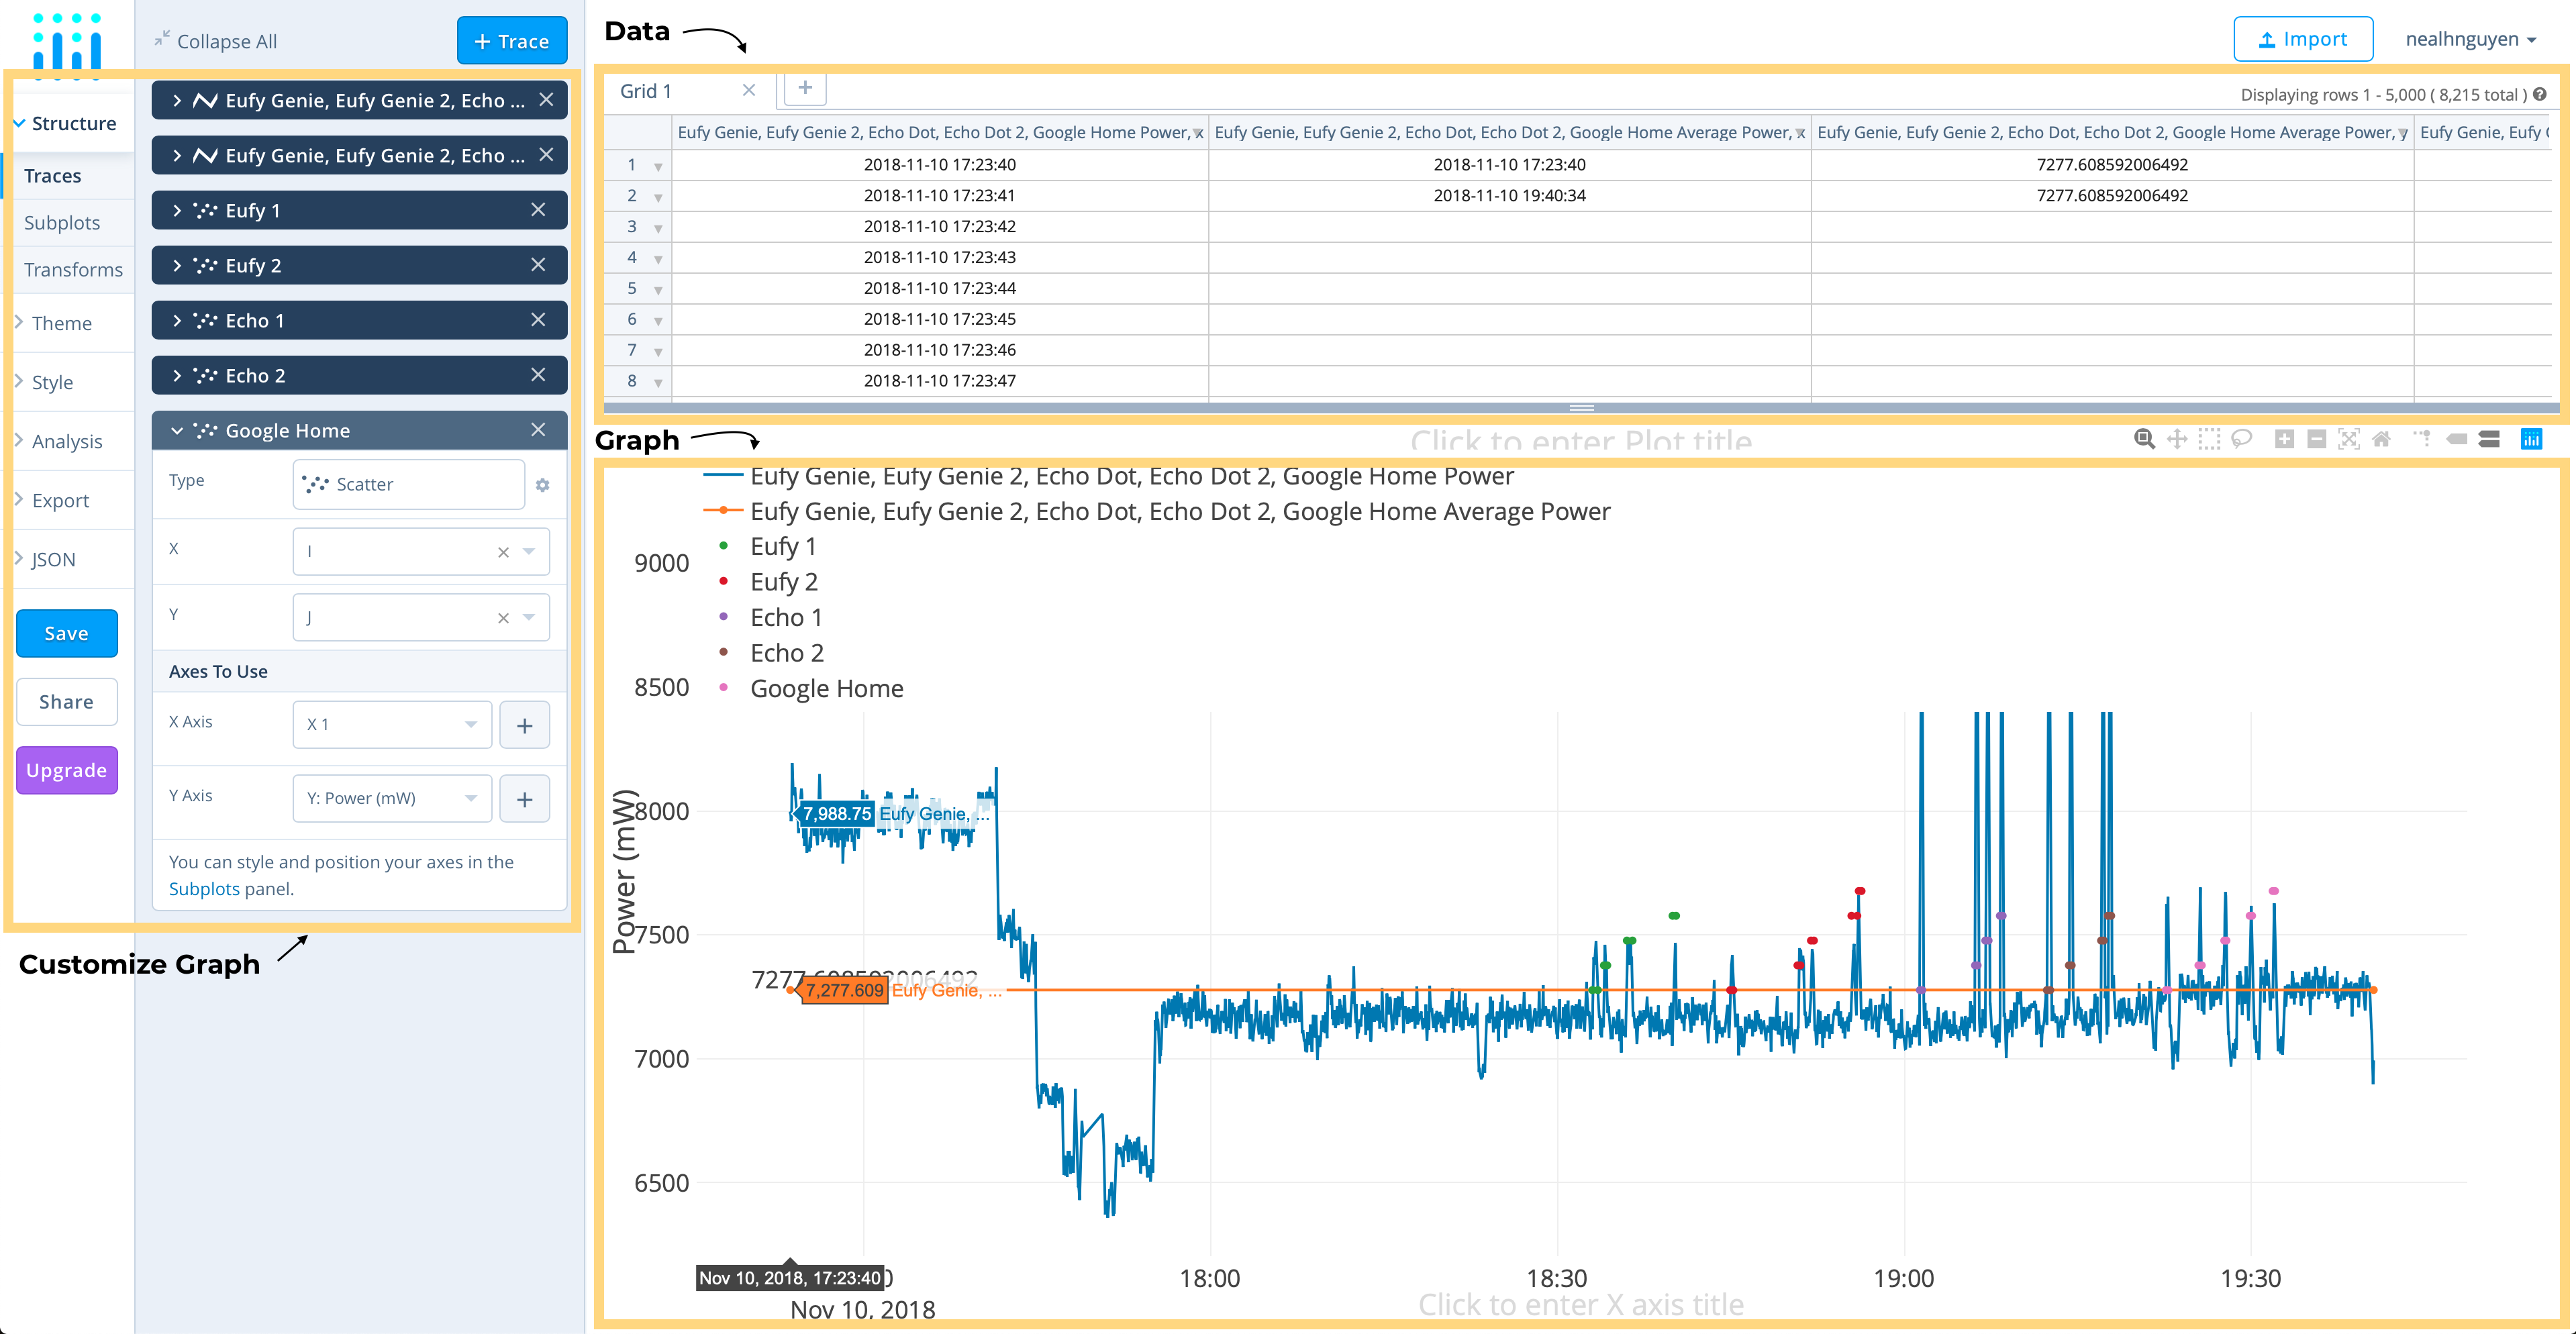
\includegraphics[width=1\textwidth]{figures/plotlyEdit.png}
    \caption{Screen to edit saved Plotly graphs containing an edit tool bar, the graph data, and the graph.}
    \label{fig:plotlyEdit}
\end{figure}

\noindent
\begin{minipage}{\textwidth}
    \begin{lstlisting}[language=SQL, label={lst:rollup},caption={Efficient SQL query to obtain total Network throughput at each second.}]
    def throughput_query_in_range(db_connection, device, start_time, end_time):
    sql_query = """
        SELECT
            time,
            CASE WHEN type IS NULL THEN 'total' ELSE type END type,
            SUM(size) AS total_throughput
        FROM ip_log.ip
        WHERE
            time BETWEEN '%s' AND '%s' AND
            (source = '%s' OR destination = '%s')
        GROUP BY time, type WITH ROLLUP;
    """ % (start_time, end_time, ip[device], ip[device])

    dataframe = pd.read_sql_query(sql_query, db_connection)

    return dataframe
    \end{lstlisting}
\end{minipage}

To reduce local computation, the grapher offloads work to the server through an SQL query. ROLLUP provides nested queries and causes the query to sum up the data by time for each type of packet. When querying for network data, the grapher performs an SQL ROLLUP to sum the incoming and outgoing network throughput to obtain the total throughput. This query is formatted as shown in Listing \ref{lst:rollup}.

To simplify data handling in the grapher, the grapher stores queried data into Pandas \cite{pandas}. Pandas is the industry standard library for dealing with tabular data. It integrates with SQL and has builtin functions to query directly from a database into a Pandas object. Pandas provides easy key, value scheme for indexing by column or row and for parsing the data.

\begin{figure}[H]
    \centering
    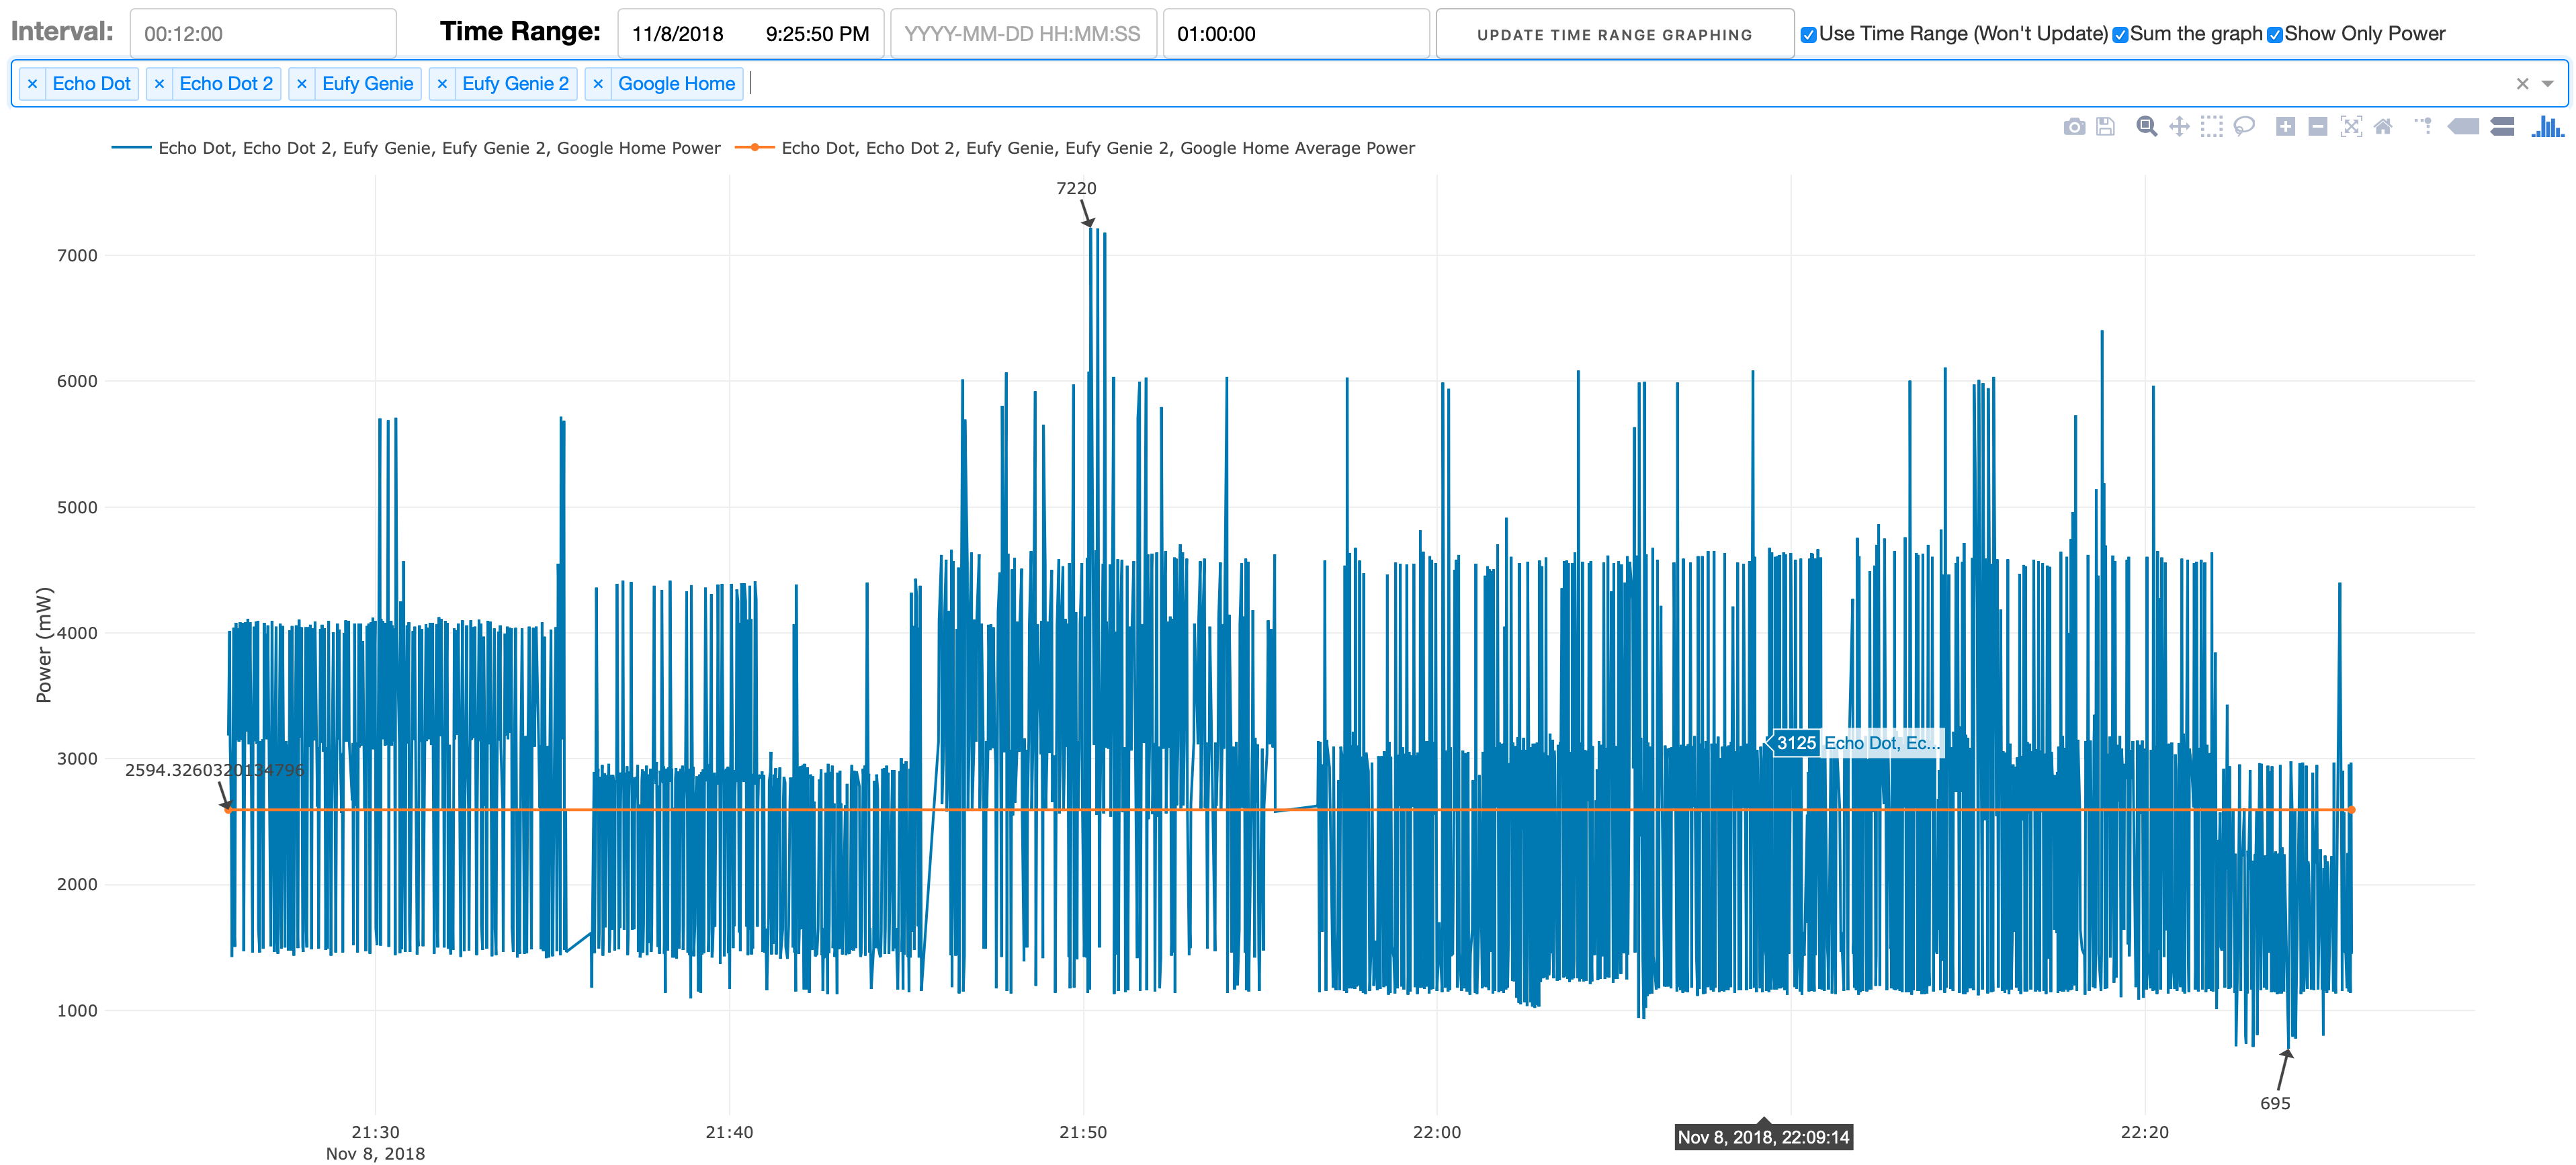
\includegraphics[width=1\textwidth]{figures/noninterpolated.png}
    \caption{Summed power traces without interpolation.}
    \label{fig:noninterpolated}
\end{figure}

\begin{figure}[H]
    \centering
    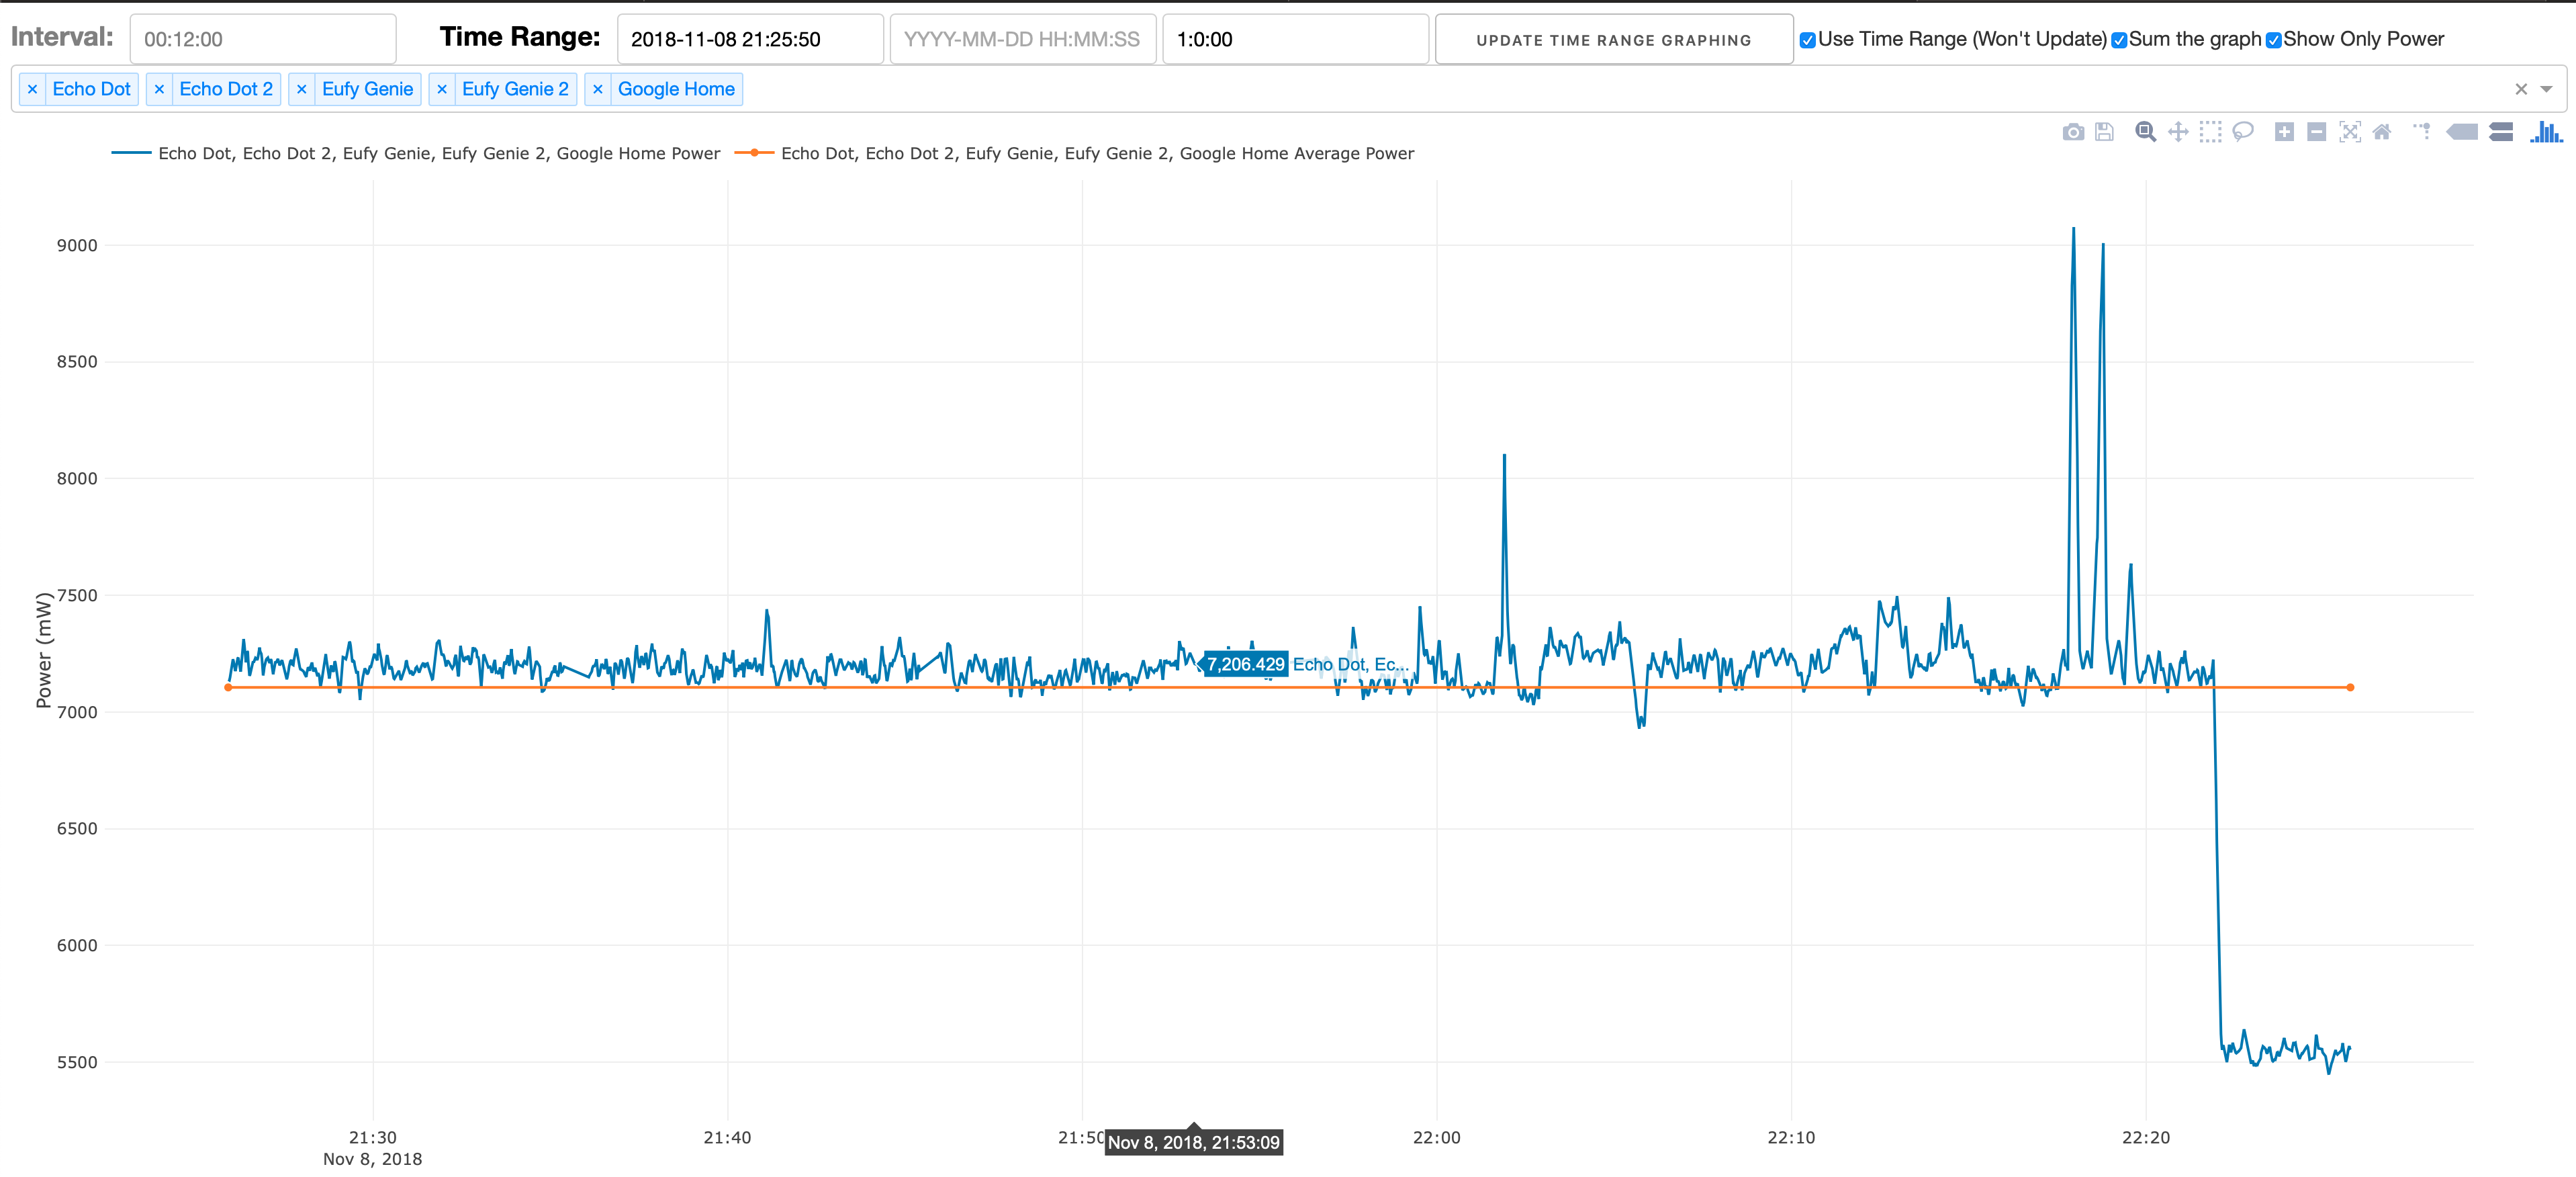
\includegraphics[width=1\textwidth]{figures/interpolated.png}
    \caption{Summed power traces with interpolation.}
    \label{fig:interpolated}
\end{figure}

The grapher can also sum all power traces into one single trace. Originally, when summing the graphs, it would add the two Pandas data frames that represent each trace, and graph the result, shown in Figure \ref{fig:noninterpolated}. However, the WeMo does not always sample every second. This is an issue if, at some time, one device X has a power point, but another device does not. The summation counts the empty data point as 0, resulting in an erroneous sum for certain frames. This was solved by interpolating data for every second for each device before summing data frames, with a built-in Pandas feature. Interpolation is shown in \ref{fig:interpolated} as a graph.

\subsubsection{Visual Takeaway}
This tool created most of the images shown in Chapter \ref{Results}. A few other researchers, including Frawley, have used this tool for data visualization. The grapher provides real-time or historical graphs on any device in the database with little effort. Additional features from Plotly also provides an easy way to format graphs for presentations or papers.

The summation feature can simplify the graph and provide a more holistic view of power usage, making it easier to spot patterns. In this paper, the summation feature is used to simulate the concept of a household's ``powerline'' where all energy usage is be summed up into one power meter.

\subsubsection{Limitations}
As this tool was created entirely for research purposes, there are some edge cases that it fails to handle.

When the database has too many connections, the grapher refuses to connect, and the grapher will not work. When graphing in real time, the grapher makes a new connection for each query. If a query hangs in the graphing tool in live mode, connections can quickly build up as the grapher continually makes a new connection every second without the previous queries closing.

The graphing tool also slows as the time frame increases. We have noticed a slow down for queries with time frames longer than seven hours. In the static graphing mode, the tool slows down before graphing the information. However, in real time graphing mode, the tool makes many slow queries, eventually causing too many connections to the database and undefined behavior.

The graphing tool uses a lookup table that maps the IP address of the device to the corresponding name given to the WeMos. Because we manually create the lookup table, when any of the IoT device's IP changes, the graphing tool is not able to find the device. In some cases, this causes the graphing tool to crash. To solve this, the user must manually change the IP addresses defined in the lookup table in lines 23-39 shown in Listing \ref{lst:ipLookup}.

\begin{minipage}{\textwidth}
    \begin{lstlisting}[label={lst:ipLookup},caption={IP lookup table in real time IoT grapher.}]
    #region IP Addresses of all devices we are tracking
    ip = {
        'Chromecast':       '192.168.12.77',
        'Echo Dot 2':       '10.42.0.132',
        'Echo Dot':         '10.42.0.150',
        'Eufy Genie':       '10.42.0.223',
        'Eufy Genie 2':     '10.42.0.172',
        'Fire Stick':       '192.168.12.113',
        'Google Home':      '10.42.0.236',
        'IP Camera':        '192.168.12.58',
        'Nintendo Switch':  '192.168.12.160',
        'Roku':             '192.168.12.68',
        'Samsung Hub':      '192.168.12.100',
        'Samsung TV':       '192.168.12.191',
        'Smart Light':      '192.168.12.27',
        'Xbox':             '192.168.12.251',
        'Echo Show':        '192.168.12.122',
        'Appliance':        '192.168.12.122',
        'Appliance1':        '192.168.12.122',
    }
    \end{lstlisting}
\end{minipage}
